
% \documentclass{article} % For LaTeX2e
% \usepackage{iclr2027_conference,times}

% % Optional math commands from https://github.com/goodfeli/dlbook_notation.
% %%%%% NEW MATH DEFINITIONS %%%%%

\usepackage{amsmath,amsfonts,bm}

% Mark sections of captions for referring to divisions of figures
\newcommand{\figleft}{{\em (Left)}}
\newcommand{\figcenter}{{\em (Center)}}
\newcommand{\figright}{{\em (Right)}}
\newcommand{\figtop}{{\em (Top)}}
\newcommand{\figbottom}{{\em (Bottom)}}
\newcommand{\captiona}{{\em (a)}}
\newcommand{\captionb}{{\em (b)}}
\newcommand{\captionc}{{\em (c)}}
\newcommand{\captiond}{{\em (d)}}

% Highlight a newly defined term
\newcommand{\newterm}[1]{{\bf #1}}


% Figure reference, lower-case.
\def\figref#1{figure~\ref{#1}}
% Figure reference, capital. For start of sentence
\def\Figref#1{Figure~\ref{#1}}
\def\twofigref#1#2{figures \ref{#1} and \ref{#2}}
\def\quadfigref#1#2#3#4{figures \ref{#1}, \ref{#2}, \ref{#3} and \ref{#4}}
% Section reference, lower-case.
\def\secref#1{section~\ref{#1}}
% Section reference, capital.
\def\Secref#1{Section~\ref{#1}}
% Reference to two sections.
\def\twosecrefs#1#2{sections \ref{#1} and \ref{#2}}
% Reference to three sections.
\def\secrefs#1#2#3{sections \ref{#1}, \ref{#2} and \ref{#3}}
% Reference to an equation, lower-case.
\def\eqref#1{equation~\ref{#1}}
% Reference to an equation, upper case
\def\Eqref#1{Equation~\ref{#1}}
% A raw reference to an equation---avoid using if possible
\def\plaineqref#1{\ref{#1}}
% Reference to a chapter, lower-case.
\def\chapref#1{chapter~\ref{#1}}
% Reference to an equation, upper case.
\def\Chapref#1{Chapter~\ref{#1}}
% Reference to a range of chapters
\def\rangechapref#1#2{chapters\ref{#1}--\ref{#2}}
% Reference to an algorithm, lower-case.
\def\algref#1{algorithm~\ref{#1}}
% Reference to an algorithm, upper case.
\def\Algref#1{Algorithm~\ref{#1}}
\def\twoalgref#1#2{algorithms \ref{#1} and \ref{#2}}
\def\Twoalgref#1#2{Algorithms \ref{#1} and \ref{#2}}
% Reference to a part, lower case
\def\partref#1{part~\ref{#1}}
% Reference to a part, upper case
\def\Partref#1{Part~\ref{#1}}
\def\twopartref#1#2{parts \ref{#1} and \ref{#2}}

\def\ceil#1{\lceil #1 \rceil}
\def\floor#1{\lfloor #1 \rfloor}
\def\1{\bm{1}}
\newcommand{\train}{\mathcal{D}}
\newcommand{\valid}{\mathcal{D_{\mathrm{valid}}}}
\newcommand{\test}{\mathcal{D_{\mathrm{test}}}}

\def\eps{{\epsilon}}


% Random variables
\def\reta{{\textnormal{$\eta$}}}
\def\ra{{\textnormal{a}}}
\def\rb{{\textnormal{b}}}
\def\rc{{\textnormal{c}}}
\def\rd{{\textnormal{d}}}
\def\re{{\textnormal{e}}}
\def\rf{{\textnormal{f}}}
\def\rg{{\textnormal{g}}}
\def\rh{{\textnormal{h}}}
\def\ri{{\textnormal{i}}}
\def\rj{{\textnormal{j}}}
\def\rk{{\textnormal{k}}}
\def\rl{{\textnormal{l}}}
% rm is already a command, just don't name any random variables m
\def\rn{{\textnormal{n}}}
\def\ro{{\textnormal{o}}}
\def\rp{{\textnormal{p}}}
\def\rq{{\textnormal{q}}}
\def\rr{{\textnormal{r}}}
\def\rs{{\textnormal{s}}}
\def\rt{{\textnormal{t}}}
\def\ru{{\textnormal{u}}}
\def\rv{{\textnormal{v}}}
\def\rw{{\textnormal{w}}}
\def\rx{{\textnormal{x}}}
\def\ry{{\textnormal{y}}}
\def\rz{{\textnormal{z}}}

% Random vectors
\def\rvepsilon{{\mathbf{\epsilon}}}
\def\rvtheta{{\mathbf{\theta}}}
\def\rva{{\mathbf{a}}}
\def\rvb{{\mathbf{b}}}
\def\rvc{{\mathbf{c}}}
\def\rvd{{\mathbf{d}}}
\def\rve{{\mathbf{e}}}
\def\rvf{{\mathbf{f}}}
\def\rvg{{\mathbf{g}}}
\def\rvh{{\mathbf{h}}}
\def\rvu{{\mathbf{i}}}
\def\rvj{{\mathbf{j}}}
\def\rvk{{\mathbf{k}}}
\def\rvl{{\mathbf{l}}}
\def\rvm{{\mathbf{m}}}
\def\rvn{{\mathbf{n}}}
\def\rvo{{\mathbf{o}}}
\def\rvp{{\mathbf{p}}}
\def\rvq{{\mathbf{q}}}
\def\rvr{{\mathbf{r}}}
\def\rvs{{\mathbf{s}}}
\def\rvt{{\mathbf{t}}}
\def\rvu{{\mathbf{u}}}
\def\rvv{{\mathbf{v}}}
\def\rvw{{\mathbf{w}}}
\def\rvx{{\mathbf{x}}}
\def\rvy{{\mathbf{y}}}
\def\rvz{{\mathbf{z}}}

% Elements of random vectors
\def\erva{{\textnormal{a}}}
\def\ervb{{\textnormal{b}}}
\def\ervc{{\textnormal{c}}}
\def\ervd{{\textnormal{d}}}
\def\erve{{\textnormal{e}}}
\def\ervf{{\textnormal{f}}}
\def\ervg{{\textnormal{g}}}
\def\ervh{{\textnormal{h}}}
\def\ervi{{\textnormal{i}}}
\def\ervj{{\textnormal{j}}}
\def\ervk{{\textnormal{k}}}
\def\ervl{{\textnormal{l}}}
\def\ervm{{\textnormal{m}}}
\def\ervn{{\textnormal{n}}}
\def\ervo{{\textnormal{o}}}
\def\ervp{{\textnormal{p}}}
\def\ervq{{\textnormal{q}}}
\def\ervr{{\textnormal{r}}}
\def\ervs{{\textnormal{s}}}
\def\ervt{{\textnormal{t}}}
\def\ervu{{\textnormal{u}}}
\def\ervv{{\textnormal{v}}}
\def\ervw{{\textnormal{w}}}
\def\ervx{{\textnormal{x}}}
\def\ervy{{\textnormal{y}}}
\def\ervz{{\textnormal{z}}}

% Random matrices
\def\rmA{{\mathbf{A}}}
\def\rmB{{\mathbf{B}}}
\def\rmC{{\mathbf{C}}}
\def\rmD{{\mathbf{D}}}
\def\rmE{{\mathbf{E}}}
\def\rmF{{\mathbf{F}}}
\def\rmG{{\mathbf{G}}}
\def\rmH{{\mathbf{H}}}
\def\rmI{{\mathbf{I}}}
\def\rmJ{{\mathbf{J}}}
\def\rmK{{\mathbf{K}}}
\def\rmL{{\mathbf{L}}}
\def\rmM{{\mathbf{M}}}
\def\rmN{{\mathbf{N}}}
\def\rmO{{\mathbf{O}}}
\def\rmP{{\mathbf{P}}}
\def\rmQ{{\mathbf{Q}}}
\def\rmR{{\mathbf{R}}}
\def\rmS{{\mathbf{S}}}
\def\rmT{{\mathbf{T}}}
\def\rmU{{\mathbf{U}}}
\def\rmV{{\mathbf{V}}}
\def\rmW{{\mathbf{W}}}
\def\rmX{{\mathbf{X}}}
\def\rmY{{\mathbf{Y}}}
\def\rmZ{{\mathbf{Z}}}

% Elements of random matrices
\def\ermA{{\textnormal{A}}}
\def\ermB{{\textnormal{B}}}
\def\ermC{{\textnormal{C}}}
\def\ermD{{\textnormal{D}}}
\def\ermE{{\textnormal{E}}}
\def\ermF{{\textnormal{F}}}
\def\ermG{{\textnormal{G}}}
\def\ermH{{\textnormal{H}}}
\def\ermI{{\textnormal{I}}}
\def\ermJ{{\textnormal{J}}}
\def\ermK{{\textnormal{K}}}
\def\ermL{{\textnormal{L}}}
\def\ermM{{\textnormal{M}}}
\def\ermN{{\textnormal{N}}}
\def\ermO{{\textnormal{O}}}
\def\ermP{{\textnormal{P}}}
\def\ermQ{{\textnormal{Q}}}
\def\ermR{{\textnormal{R}}}
\def\ermS{{\textnormal{S}}}
\def\ermT{{\textnormal{T}}}
\def\ermU{{\textnormal{U}}}
\def\ermV{{\textnormal{V}}}
\def\ermW{{\textnormal{W}}}
\def\ermX{{\textnormal{X}}}
\def\ermY{{\textnormal{Y}}}
\def\ermZ{{\textnormal{Z}}}

% Vectors
\def\vzero{{\bm{0}}}
\def\vone{{\bm{1}}}
\def\vmu{{\bm{\mu}}}
\def\vtheta{{\bm{\theta}}}
\def\va{{\bm{a}}}
\def\vb{{\bm{b}}}
\def\vc{{\bm{c}}}
\def\vd{{\bm{d}}}
\def\ve{{\bm{e}}}
\def\vf{{\bm{f}}}
\def\vg{{\bm{g}}}
\def\vh{{\bm{h}}}
\def\vi{{\bm{i}}}
\def\vj{{\bm{j}}}
\def\vk{{\bm{k}}}
\def\vl{{\bm{l}}}
\def\vm{{\bm{m}}}
\def\vn{{\bm{n}}}
\def\vo{{\bm{o}}}
\def\vp{{\bm{p}}}
\def\vq{{\bm{q}}}
\def\vr{{\bm{r}}}
\def\vs{{\bm{s}}}
\def\vt{{\bm{t}}}
\def\vu{{\bm{u}}}
\def\vv{{\bm{v}}}
\def\vw{{\bm{w}}}
\def\vx{{\bm{x}}}
\def\vy{{\bm{y}}}
\def\vz{{\bm{z}}}

% Elements of vectors
\def\evalpha{{\alpha}}
\def\evbeta{{\beta}}
\def\evepsilon{{\epsilon}}
\def\evlambda{{\lambda}}
\def\evomega{{\omega}}
\def\evmu{{\mu}}
\def\evpsi{{\psi}}
\def\evsigma{{\sigma}}
\def\evtheta{{\theta}}
\def\eva{{a}}
\def\evb{{b}}
\def\evc{{c}}
\def\evd{{d}}
\def\eve{{e}}
\def\evf{{f}}
\def\evg{{g}}
\def\evh{{h}}
\def\evi{{i}}
\def\evj{{j}}
\def\evk{{k}}
\def\evl{{l}}
\def\evm{{m}}
\def\evn{{n}}
\def\evo{{o}}
\def\evp{{p}}
\def\evq{{q}}
\def\evr{{r}}
\def\evs{{s}}
\def\evt{{t}}
\def\evu{{u}}
\def\evv{{v}}
\def\evw{{w}}
\def\evx{{x}}
\def\evy{{y}}
\def\evz{{z}}

% Matrix
\def\mA{{\bm{A}}}
\def\mB{{\bm{B}}}
\def\mC{{\bm{C}}}
\def\mD{{\bm{D}}}
\def\mE{{\bm{E}}}
\def\mF{{\bm{F}}}
\def\mG{{\bm{G}}}
\def\mH{{\bm{H}}}
\def\mI{{\bm{I}}}
\def\mJ{{\bm{J}}}
\def\mK{{\bm{K}}}
\def\mL{{\bm{L}}}
\def\mM{{\bm{M}}}
\def\mN{{\bm{N}}}
\def\mO{{\bm{O}}}
\def\mP{{\bm{P}}}
\def\mQ{{\bm{Q}}}
\def\mR{{\bm{R}}}
\def\mS{{\bm{S}}}
\def\mT{{\bm{T}}}
\def\mU{{\bm{U}}}
\def\mV{{\bm{V}}}
\def\mW{{\bm{W}}}
\def\mX{{\bm{X}}}
\def\mY{{\bm{Y}}}
\def\mZ{{\bm{Z}}}
\def\mBeta{{\bm{\beta}}}
\def\mPhi{{\bm{\Phi}}}
\def\mLambda{{\bm{\Lambda}}}
\def\mSigma{{\bm{\Sigma}}}

% Tensor
\DeclareMathAlphabet{\mathsfit}{\encodingdefault}{\sfdefault}{m}{sl}
\SetMathAlphabet{\mathsfit}{bold}{\encodingdefault}{\sfdefault}{bx}{n}
\newcommand{\tens}[1]{\bm{\mathsfit{#1}}}
\def\tA{{\tens{A}}}
\def\tB{{\tens{B}}}
\def\tC{{\tens{C}}}
\def\tD{{\tens{D}}}
\def\tE{{\tens{E}}}
\def\tF{{\tens{F}}}
\def\tG{{\tens{G}}}
\def\tH{{\tens{H}}}
\def\tI{{\tens{I}}}
\def\tJ{{\tens{J}}}
\def\tK{{\tens{K}}}
\def\tL{{\tens{L}}}
\def\tM{{\tens{M}}}
\def\tN{{\tens{N}}}
\def\tO{{\tens{O}}}
\def\tP{{\tens{P}}}
\def\tQ{{\tens{Q}}}
\def\tR{{\tens{R}}}
\def\tS{{\tens{S}}}
\def\tT{{\tens{T}}}
\def\tU{{\tens{U}}}
\def\tV{{\tens{V}}}
\def\tW{{\tens{W}}}
\def\tX{{\tens{X}}}
\def\tY{{\tens{Y}}}
\def\tZ{{\tens{Z}}}


% Graph
\def\gA{{\mathcal{A}}}
\def\gB{{\mathcal{B}}}
\def\gC{{\mathcal{C}}}
\def\gD{{\mathcal{D}}}
\def\gE{{\mathcal{E}}}
\def\gF{{\mathcal{F}}}
\def\gG{{\mathcal{G}}}
\def\gH{{\mathcal{H}}}
\def\gI{{\mathcal{I}}}
\def\gJ{{\mathcal{J}}}
\def\gK{{\mathcal{K}}}
\def\gL{{\mathcal{L}}}
\def\gM{{\mathcal{M}}}
\def\gN{{\mathcal{N}}}
\def\gO{{\mathcal{O}}}
\def\gP{{\mathcal{P}}}
\def\gQ{{\mathcal{Q}}}
\def\gR{{\mathcal{R}}}
\def\gS{{\mathcal{S}}}
\def\gT{{\mathcal{T}}}
\def\gU{{\mathcal{U}}}
\def\gV{{\mathcal{V}}}
\def\gW{{\mathcal{W}}}
\def\gX{{\mathcal{X}}}
\def\gY{{\mathcal{Y}}}
\def\gZ{{\mathcal{Z}}}

% Sets
\def\sA{{\mathbb{A}}}
\def\sB{{\mathbb{B}}}
\def\sC{{\mathbb{C}}}
\def\sD{{\mathbb{D}}}
% Don't use a set called E, because this would be the same as our symbol
% for expectation.
\def\sF{{\mathbb{F}}}
\def\sG{{\mathbb{G}}}
\def\sH{{\mathbb{H}}}
\def\sI{{\mathbb{I}}}
\def\sJ{{\mathbb{J}}}
\def\sK{{\mathbb{K}}}
\def\sL{{\mathbb{L}}}
\def\sM{{\mathbb{M}}}
\def\sN{{\mathbb{N}}}
\def\sO{{\mathbb{O}}}
\def\sP{{\mathbb{P}}}
\def\sQ{{\mathbb{Q}}}
\def\sR{{\mathbb{R}}}
\def\sS{{\mathbb{S}}}
\def\sT{{\mathbb{T}}}
\def\sU{{\mathbb{U}}}
\def\sV{{\mathbb{V}}}
\def\sW{{\mathbb{W}}}
\def\sX{{\mathbb{X}}}
\def\sY{{\mathbb{Y}}}
\def\sZ{{\mathbb{Z}}}

% Entries of a matrix
\def\emLambda{{\Lambda}}
\def\emA{{A}}
\def\emB{{B}}
\def\emC{{C}}
\def\emD{{D}}
\def\emE{{E}}
\def\emF{{F}}
\def\emG{{G}}
\def\emH{{H}}
\def\emI{{I}}
\def\emJ{{J}}
\def\emK{{K}}
\def\emL{{L}}
\def\emM{{M}}
\def\emN{{N}}
\def\emO{{O}}
\def\emP{{P}}
\def\emQ{{Q}}
\def\emR{{R}}
\def\emS{{S}}
\def\emT{{T}}
\def\emU{{U}}
\def\emV{{V}}
\def\emW{{W}}
\def\emX{{X}}
\def\emY{{Y}}
\def\emZ{{Z}}
\def\emSigma{{\Sigma}}

% entries of a tensor
% Same font as tensor, without \bm wrapper
\newcommand{\etens}[1]{\mathsfit{#1}}
\def\etLambda{{\etens{\Lambda}}}
\def\etA{{\etens{A}}}
\def\etB{{\etens{B}}}
\def\etC{{\etens{C}}}
\def\etD{{\etens{D}}}
\def\etE{{\etens{E}}}
\def\etF{{\etens{F}}}
\def\etG{{\etens{G}}}
\def\etH{{\etens{H}}}
\def\etI{{\etens{I}}}
\def\etJ{{\etens{J}}}
\def\etK{{\etens{K}}}
\def\etL{{\etens{L}}}
\def\etM{{\etens{M}}}
\def\etN{{\etens{N}}}
\def\etO{{\etens{O}}}
\def\etP{{\etens{P}}}
\def\etQ{{\etens{Q}}}
\def\etR{{\etens{R}}}
\def\etS{{\etens{S}}}
\def\etT{{\etens{T}}}
\def\etU{{\etens{U}}}
\def\etV{{\etens{V}}}
\def\etW{{\etens{W}}}
\def\etX{{\etens{X}}}
\def\etY{{\etens{Y}}}
\def\etZ{{\etens{Z}}}

% The true underlying data generating distribution
\newcommand{\pdata}{p_{\rm{data}}}
% The empirical distribution defined by the training set
\newcommand{\ptrain}{\hat{p}_{\rm{data}}}
\newcommand{\Ptrain}{\hat{P}_{\rm{data}}}
% The model distribution
\newcommand{\pmodel}{p_{\rm{model}}}
\newcommand{\Pmodel}{P_{\rm{model}}}
\newcommand{\ptildemodel}{\tilde{p}_{\rm{model}}}
% Stochastic autoencoder distributions
\newcommand{\pencode}{p_{\rm{encoder}}}
\newcommand{\pdecode}{p_{\rm{decoder}}}
\newcommand{\precons}{p_{\rm{reconstruct}}}

\newcommand{\laplace}{\mathrm{Laplace}} % Laplace distribution

\newcommand{\E}{\mathbb{E}}
\newcommand{\Ls}{\mathcal{L}}
\newcommand{\R}{\mathbb{R}}
\newcommand{\emp}{\tilde{p}}
\newcommand{\lr}{\alpha}
\newcommand{\reg}{\lambda}
\newcommand{\rect}{\mathrm{rectifier}}
\newcommand{\softmax}{\mathrm{softmax}}
\newcommand{\sigmoid}{\sigma}
\newcommand{\softplus}{\zeta}
\newcommand{\KL}{D_{\mathrm{KL}}}
\newcommand{\Var}{\mathrm{Var}}
\newcommand{\standarderror}{\mathrm{SE}}
\newcommand{\Cov}{\mathrm{Cov}}
% Wolfram Mathworld says $L^2$ is for function spaces and $\ell^2$ is for vectors
% But then they seem to use $L^2$ for vectors throughout the site, and so does
% wikipedia.
\newcommand{\normlzero}{L^0}
\newcommand{\normlone}{L^1}
\newcommand{\normltwo}{L^2}
\newcommand{\normlp}{L^p}
\newcommand{\normmax}{L^\infty}

\newcommand{\parents}{Pa} % See usage in notation.tex. Chosen to match Daphne's book.

\DeclareMathOperator*{\argmax}{arg\,max}
\DeclareMathOperator*{\argmin}{arg\,min}

\DeclareMathOperator{\sign}{sign}
\DeclareMathOperator{\Tr}{Tr}
\let\ab\allowbreak


\newcommand{\vphi}{\boldsymbol{\phi}}
\newcommand{\vsigma}{\boldsymbol{\sigma}}
% \usepackage{float}
% \floatstyle{ruled}
% \newfloat{algorithm}{tbp}{loa}
% \floatname{algorithm}{Algorithm}
% \usepackage{capt-of}
% \usepackage{hyperref}
% \usepackage{url}
% \usepackage{booktabs}
% \usepackage{graphicx}
% \usepackage{colortbl}
% \usepackage{wrapfig}
% \usepackage{svg}
% \usepackage{enumitem}
% \usepackage{cleveref}

% \Crefname{equation}{Equation}{Equations}
% \crefname{equation}{Eq.}{Eqs.}
% \Crefname{figure}{Figure}{Figures}
% \crefname{figure}{Fig.}{Figs.}
% \Crefname{table}{Table}{Tables}
% \crefname{table}{Table}{Tables}
% \Crefname{algorithm}{Algorithm}{Algorithms}
% \crefname{algorithm}{Alg.}{Algs.}

% % Lightweight pseudocode used by the appendix algorithms. Keeping this
% % local definition avoids an additional algorithmic package dependency.
% \newenvironment{vsfalgorithmic}{%
%   \begingroup
%   \footnotesize
%   \raggedright
%   \setlength{\parindent}{0pt}%
%   \setlength{\parskip}{0.2em}%
% }{%
%   \par\endgroup
% }
% \newcommand{\VSFInput}{\par\noindent\textbf{Input:}~}
% \newcommand{\VSFOutput}{\par\noindent\textbf{Output:}~}
% \newcommand{\VSFState}{\par\noindent}
% \newcommand{\VSFWhile}[1]{%
%   \par\noindent\textbf{while} #1 \textbf{do}\par
%   \begingroup\addtolength{\leftskip}{1em}%
% }
% \newcommand{\VSFEndWhile}{%
%   \par\endgroup\noindent\textbf{end while}%
% }
% \newcommand{\VSFFor}[1]{%
%   \par\noindent\textbf{for} #1 \textbf{do}\par
%   \begingroup\addtolength{\leftskip}{1em}%
% }
% \newcommand{\VSFEndFor}{%
%   \par\endgroup\noindent\textbf{end for}%
% }

% \newcommand{\Minseon}[1]{\textcolor{blue}{Minseon: #1}}

% \usepackage{bm}
% \usepackage{tcolorbox}
% \tcbuselibrary{skins}

% \definecolor{sand}{RGB}{248,245,235}  % very light sand
% \definecolor{sandborder}{RGB}{220,215,200}
% \definecolor{darkblue}{RGB}{40,70,140}   % softer
% \definecolor{parchment}{RGB}{252,249,240}
% \definecolor{parchmentborder}{RGB}{222,215,195}
% \definecolor{sage}{RGB}{244,248,244}
% \definecolor{sageborder}{RGB}{200,210,200}
% \definecolor{lavender}{RGB}{247,246,250}
% \definecolor{lavenderborder}{RGB}{210,205,225}
% \definecolor{riskbg}{RGB}{255,246,246}
% \definecolor{riskborder}{RGB}{205,105,105}


% \definecolor{resultDPBg}{RGB}{242,247,255}
% \definecolor{resultRosslerBg}{RGB}{242,250,244}
% \definecolor{resultLorenzBg}{RGB}{255,247,235}
% \definecolor{resultRuntimeBg}{RGB}{245,240,252}
% \newlength{\resultHeaderGap}
% \setlength{\resultHeaderGap}{\dimexpr\aboverulesep+\cmidrulewidth+\belowrulesep\relax}
% \newcommand{\resultRuntimeHeaderFill}[1]{%
%   \noalign{\vskip-\dimexpr 2\aboverulesep+\cmidrulewidth+2\belowrulesep\relax}%
%   \arrayrulecolor{resultRuntimeBg}%
%   \cmidrule[\resultHeaderGap]{#1-#1}%
%   \arrayrulecolor{black}%
% }

% \newtheorem{vsftheorem}{Theorem}[section]
% \newtheorem{vsfcorollary}[vsftheorem]{Corollary}
% \newtheorem{vsfproposition}[vsftheorem]{Proposition}
% \numberwithin{equation}{section}
% \setcounter{equation}{0}


% \providecommand{\resultpm}[2]{\ensuremath{#1 \mathbin{\pm} #2}}
% \providecommand{\bestresultpm}[2]{\ensuremath{\mathbf{#1} \mathbin{\pm} #2}}
% \providecommand{\fullbestresultpm}[2]{\ensuremath{\boldsymbol{#1 \mathbin{\pm} #2}}}
% \providecommand{\secondbestresultpm}[2]{\ensuremath{\underline{#1 \mathbin{\pm} #2}}}
% \providecommand{\DoublePendulumChaoticInstance}{02}

% %\title{Variational Streaming Flow for Probabilistic Forecasting}

% \title{Variational Streaming Flow: Probabilistic Forecasting in Physical Time}

% % Authors must not appear in the submitted version. They should be hidden
% % as long as the \iclrfinalcopy macro remains commented out below.
% % Non-anonymous submissions will be rejected without review.

% \author{Antiquus S.~Hippocampus, Natalia Cerebro \& Amelie P. Amygdale \thanks{ Use footnote for providing further information
% about author (webpage, alternative address)---\emph{not} for acknowledging
% funding agencies.  Funding acknowledgements go at the end of the paper.} \\
% Department of Computer Science\\
% Cranberry-Lemon University\\
% Pittsburgh, PA 15213, USA \\
% \texttt{\{hippo,brain,jen\}@cs.cranberry-lemon.edu} \\
% \And
% Ji Q. Ren \& Yevgeny LeNet \\
% Department of Computational Neuroscience \\
% University of the Witwatersrand \\
% Joburg, South Africa \\
% \texttt{\{robot,net\}@wits.ac.za} \\
% \AND
% Coauthor \\
% Affiliation \\
% Address \\
% \texttt{email}
% }

% % The \author macro works with any number of authors. There are two commands
% % used to separate the names and addresses of multiple authors: \And and \AND.
% %
% % Using \And between authors leaves it to \LaTeX{} to determine where to break
% % the lines. Using \AND forces a linebreak at that point. So, if \LaTeX{}
% % puts 3 of 4 authors names on the first line, and the last on the second
% % line, try using \AND instead of \And before the third author name.

% \newcommand{\fix}{\marginpar{FIX}}
% \newcommand{\new}{\marginpar{NEW}}
% \newcommand{\hans}[1]{\textcolor{blue}{hans: #1}}

% \newcommand{\pan}[1]{\textcolor{red}{PL: #1}}
% %\iclrfinalcopy % Uncomment for camera-ready version, but NOT for submission.
% \begin{document}


% \maketitle

% \begin{abstract}
% Probabilistic forecasting is important for predicting complex dynamical systems because intrinsic randomness and incomplete observations can cause the same observed state to evolve into multiple plausible futures. While flow matching is a flexible approach for probabilistic forecasting, it is computationally expensive. Streaming flow (SF) reformulates this approach to model temporal evolution efficiently by learning a continuous velocity field directly in physical time. However, SF learns a deterministic velocity field. Thus, it provides only a single future trajectory for a given fixed initial state and observation history. To overcome this limitation, we introduce Variational Streaming Flow (VSF). Our approach learns a latent distribution that is conditioned on the dynamics of interest. In turn, this enables probabilistic forecasting. Importantly, we retain the computational efficiency of SF by generating in physical time. Across deterministic and stochastic dynamical systems, VSF demonstrates superior predictive accuracy and distributional fidelity. We demonstrate the advantage for both long-horizon rollouts exceeding 1,000 steps, and settings with bifurcating dynamics. Moreover, VSF can be integrated into existing Joint-Embedding Predictive Architecture (JEPA)-based world models as a plug-and-play predictor to improve temporal dynamics and goal-directed success rate in navigation, motion planning, and manipulation.
% \end{abstract}


\begin{figure}[H]
% \vspace{-0.3cm}
\vspace{-0.5cm}
  \centering
  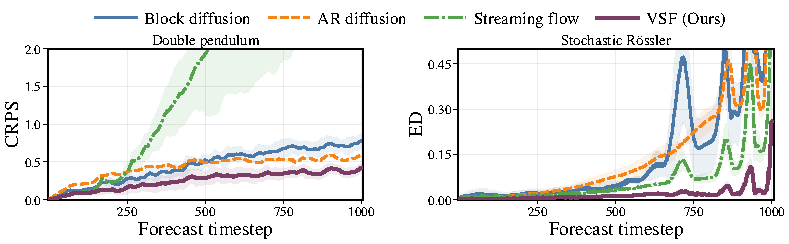
\includegraphics[width=0.95\linewidth]{figures/rollout_error_plots/combined/rollout_errors_side_by_side.pdf}
  % \vspace{-2.5em}
  \vspace{-0.8em}
\caption{Our variational streaming flow approach obtains lower forecasting error over long rollouts than standard streaming flow. Left: continuous ranked probability score (CRPS) on the deterministic double pendulum. Right: energy distance (ED) on the partially observed R\"ossler system.}
  \label{fig:main-rollout-error-curves}
  \vspace{-0.15cm}
\end{figure}




\section{Introduction}

Forecasting dynamical systems over long horizons remains challenging. Even when the dynamics are deterministic, small measurement or prediction errors can compound over a long rollout~\citep{zhang2025zero}. Predicting the entire future trajectory at once can avoid this recursive error accumulation, but this becomes an increasingly difficult learning task as the forecast horizon grows. Many real-world systems are also stochastic, which means that there can be many different future trajectories for the same sequence of observations~\citep{pfister2026stocbench}. For example, in weather forecasting~\citep{ feng2013expansion,sandu2019impacts, price2025probabilistic}, unresolved atmospheric processes can lead to different storm tracks from similar observations. In these settings, predicting just a single trajectory is insufficient for forecasting or planning. This motivates probabilistic forecasts that represent a distribution over possible futures~\citep{chua2018deep,porcher2026flow}.

Flow matching provides a flexible way to learn probabilistic forecasts over entire future trajectories~\citep{lipman2024flow,kollovieh2025tsflow}. However, generating a forecast requires integrating a learned vector field along an auxiliary flow time that is separate from the physical evolution of the system. Streaming and physical-time formulations instead evolve the predicted state directly through physical time, making long-horizon forecasting more efficient~\citep{jiang2025streaming,liu2026odeworld}. However, a standard non-latent physical-time model with a deterministic velocity field produces only one future from a fixed observed state.


To address this limitation, we introduce \emph{Variational Streaming Flow} (VSF), a probabilistic extension of physical-time flow forecasting. VSF augments the physical-time velocity field with a latent variable that is sampled once for each forecast and kept fixed throughout the rollout. This preserves the computational efficiency of streaming flow (SF) while improving long-horizon forecasting accuracy, as shown in \cref{fig:main-rollout-error-curves}. Different latent samples can also generate different future trajectories from the same observed state, allowing VSF to represent multiple possible futures.
%
During training, we use an encoder to infer the latent variable from the observed future transition and regularize its distribution toward a fixed prior~\citep{guo2025variational,eijkelboom2024variational}. At inference, we only need to sample a latent from the prior and keep it fixed throughout the rollout.

% To address this limitation, we introduce \emph{Variational Streaming Flow} (VSF). Our approach augments the physical-time velocity field with a latent variable that is sampled once for each forecast. Starting from the same observed state, different latent samples can therefore generate different future trajectories, while each trajectory still evolves directly in physical time. Figure~\ref{fig:forecasting-settings} illustrates this distinction between standard SF, which produces a single trajectory from a fixed initial state, and VSF, which can produce multiple plausible futures.
% %
% Given an observed history $\vx_{a:m}$, we summarize the history by $\vh=H(\vx_{a:m})$. The forecast then evolves according to the following latent-conditioned flow:
% %
% \begin{tcolorbox}[
% colback=parchment,
% colframe=sandborder,
% boxrule=0.3pt,
% left=8pt,
% right=8pt,
% top=3pt,
% bottom=3pt
% ]
% \begin{equation}
% \frac{d\widehat{\vx}_s}{ds}
% =
% \vv_{\vtheta}
% \left(
% \widehat{\vx}_s,s,\vh,\vz
% \right).
% \label{eq:intro_vsf}
% \end{equation}
% \end{tcolorbox}
% %
% Here, $\widehat{\vx}_s$ is the predicted system state at physical forecast time $s$, and the rollout starts from the most recent observed state $\vx_m$. The velocity field is conditioned on the observed history $\vh$ and on a latent variable $\vz$. A single $\vz$ is sampled at the beginning of the forecast and kept fixed throughout the rollout, so it can consistently influence which future trajectory the model follows. During training, we use an encoder to infer the latent variable from the observed future transition. A KL regularization term encourages the inferred latent distribution to remain close to the prior used at inference~\citep{guo2025variational,eijkelboom2024variational}. At inference, we only need to sample a latent from the prior and keep it fixed throughout the rollout.



We evaluate VSF on deterministic and partially observed stochastic dynamical systems, including chaotic systems and settings with branching futures, testing both predictive accuracy and distributional fidelity. On deterministic systems, VSF improves long-horizon predictive accuracy over DeepAR~\citep{salinas2020deepar}, diffusion- and flow-based forecasters, SF~\citep{jiang2025streaming}, and Chronos-2~\citep{ansari2025chronos}. On stochastic R\"ossler and Lorenz systems, VSF more accurately recovers the conditional distribution of long-horizon futures. We further use VSF as the predictor in a JEPA-based world model~\citep{maes2026leworldmodel}; see \cref{fig:world-model-predictor}. Across four robotics tasks, VSF improves average goal-directed planning success by $7.34\%$ over LeWM's deterministic predictor while retaining one velocity-field evaluation per imagined transition.

Our main contributions are as follows.

\begin{itemize}[leftmargin=*]

\item We introduce \emph{Variational Streaming Flow}, a variational latent
variable formulation of physical-time flow modeling in which one latent draw
conditions a full forecast rollout. It is motivated by a limitation of
non-latent physical-time flows near bifurcations, where small differences in
state can make the learned dynamics highly sensitive to perturbations
(see App.~\ref{app_motivate}).

\item We develop a variational learning framework for latent-conditioned
physical-time velocities (see \cref{sec:method}). We derive a
conditional-velocity ELBO and introduce an energy-based reconstruction over
multiple latent samples. Under posterior--prior alignment, we show that the
resulting reconstruction controls the energy distance between predicted and
true velocity distributions.

\item We evaluate VSF on deterministic and stochastic forecasting and in an
action-conditioned world model. VSF improves long-horizon predictive accuracy
and distributional fidelity, while its predictions improve goal-directed
planning and retain the efficiency of physical-time forecasting.

\end{itemize}



\begin{figure}[!t]
  \centering
  \includegraphics[
    width=0.95\linewidth,
    trim={0bp 10bp 0bp 12bp},
    clip
  ]{figures/vsf_lewm.pdf}
  \vspace{-0.8em}
\caption{
VSF can serve as a predictor in a JEPA-based world model. We replace the deterministic autoregressive predictor with an action-conditioned VSF predictor while keeping the JEPA encoder and CEM planner fixed. The encoder maps the current and goal observations into latent space. For each action sequence, VSF samples multiple latents and rolls out future trajectories. CEM compares the predicted terminal states with the goal representation and uses these costs to select a plan.
}
  \label{fig:world-model-predictor}
  % Link: https://drive.google.com/file/d/1VlHFP2pe0Q471FzFswVsvX5lGRsEucYs/view?usp=sharing
\vspace{-1em}
\end{figure}

\section{Related Work}
\label{sec:related-work}





% Flow matching provides a general framework for learning continuous
% transport dynamics between probability distributions
% ~\citep{lipman2024flow}. Recent extensions incorporate latent variables to represent uncertainty and multimodality in the learned velocity field~\citep{eijkelboom2024variational,guo2025variational}. There is also growing interest in generative methods for forecasting, where the goal is to represent a distribution over possible future trajectories rather than a single prediction.

\textbf{Probabilistic and generative forecasting.} Probabilistic time-series forecasting has traditionally modeled future uncertainty through autoregressive conditional distributions—using either deterministic states like DeepAR~\citep{salinas2020deepar} or stochastic latent variables like the Variational RNN~\citep{chung2015recurrent}. CLOVER~\citep{olivares2015clover} further refines traditional parametric forecasting by reparameterizing the coherent learning objective to better optimize distribution matching. TimeGrad instead replaces these parametric one-step distributions with an autoregressive diffusion model~\citep{rasul2021timegrad}. More recently, pretrained time-series models have enabled forecasting across datasets without task-specific training. Lag-Llama provides a probabilistic decoder-only model
~\citep{rasul2024lagllama}, while Chronos models scaled and quantized
time-series values with language-model architectures~\citep{ansari2024chronos}. Other foundation models instead use direct multi-horizon prediction, including TimesFM~\citep{das2024timesfm}, Moirai~\citep{woo2024moirai}, and the multivariate and covariate-conditioned Chronos-2~\citep{ansari2025chronos}. Such models can
also provide strong zero-shot forecasts for chaotic systems
~\citep{zhang2025zero}, but they do not explicitly parameterize the
underlying evolution as a physical-time dynamical system~\citep{karaouli2025foundational}. A complementary line of work uses diffusion and flow matching to model conditional future distributions~\citep{erichson2025flex}. Rolling Diffusion adapts the diffusion process across forecast lead time~\citep{ruhe2024rolling}, TSFlow introduces Gaussian-process priors for conditional flow matching~\citep{kollovieh2025tsflow}, and flow-based forecasting has been improved through informed probability paths~\citep{lim2025paths}, autoregressive conditional flows
~\citep{elgazzar2025flowtime}, and Bayesian-filtering-inspired transport between successive predictive distributions~\citep{huang2026sequential}. 

\textbf{Streaming and physical-time flows.} Another line of work removes the distinction between generative flow time and temporal evolution. Streaming Flow Policy treats an action trajectory itself as the flow trajectory, enabling actions to be generated and executed incrementally~\citep{jiang2025streaming}. For sequential data, \citet{lim2026flow} show that empirical flow matching can be interpreted as a memory-augmented continuous-time dynamical system whose velocity field is constructed from historical transitions. Most directly, ODEWorld introduces Physical-Time Flow, which learns a latent velocity field whose integration directly follows physical time~\citep{liu2026odeworld}.

\textbf{Stochastic world models and probabilistic planning.} Predictive uncertainty has long played a role in model-based control~\citep{watter2015embed,ha2018world,hafner2025mastering}. PETS combines probabilistic dynamics ensembles with trajectory sampling
~\citep{chua2018deep}, while PlaNet learns latent dynamics with both
deterministic and stochastic components and plans through imagined
trajectories~\citep{hafner2019planet}. Recent visual world models instead often predict directly in learned feature spaces. DINO-WM predicts future pretrained visual features under candidate actions and uses these predictions for test-time planning~\citep{zhou2025dinowm}, while LeWorldModel learns an end-to-end joint-embedding predictor for efficient latent-space planning~\citep{maes2026leworldmodel}. FlowWM explicitly addresses multimodal future uncertainty by applying flow matching in pretrained feature space~\citep{porcher2026flow}. 



{\bf Positioning.}  Streaming Flow (SF) formulates sequence generation directly in physical time
~\citep{jiang2025streaming}, but its standard construction represents residual
stochasticity through the evolving physical state; an auxiliary-latent
extension is also possible. Variational flow matching provides a mechanism for
representing multimodal velocity fields by inferring latent variables from
observed target dynamics~\citep{guo2025variational,eijkelboom2024variational}.
We bring these ideas together in \emph{Variational Streaming Flow (VSF)}, a
conditional latent variable formulation of physical-time flow modeling for
probabilistic forecasting. During training, a variational encoder associates
observed future dynamics with latent codes, while at inference a latent drawn
from the prior conditions a complete physical-time rollout from the observed
state. Thus, we view VSF not as the first latent SF model, but as a variational
latent variable formulation of SF for probabilistic forecasting.
Table~\ref{tab:vsf_positioning} summarizes this positioning.

This combination also raises a question specific to physical-time forecasting:
why is it useful to represent future-specific information outside the evolving
physical state? We illustrate one such mechanism through a simple
bifurcation example in App.~\ref{app_motivate}.


\begin{table}[!t]
\centering
\caption{
Comparison of VSF with closely related flow-based formulations.
``Physical time'' means that flow progression is identified with the
temporal evolution of the modeled sequence, rather than an artificial
generative-time coordinate.
``History-conditioned'' denotes explicit conditioning on an observed
history.
``Variational'' denotes the use of a training-time recognition model for
latent inference.
``Future-informed latent'' indicates that the latent representation is
inferred \emph{during training} from the realized target dynamics, rather than
introduced solely as an auxiliary stochastic coordinate. 
}
\label{tab:vsf_positioning}
\small
\vspace{0.2cm}
\setlength{\tabcolsep}{5pt}
\begin{tabular}{lccccc}
\toprule
Method
& Physical time
& History-cond.
& Latent
& Variational
& Future-informed latent \\
\midrule
FM/Rectified Flow
& \xmark
& \xmark
& \xmark
& \xmark
& \xmark \\

Variational Rectified FM
%\citep{guo2025variational}
& \xmark
& \xmark
& \cmark
& \cmark
& \cmark \\

SFP
%\citep{jiang2025streaming}
& \cmark
& \cmark
& \xmark
& \xmark
& \xmark \\

SFP + auxiliary latent
%\citep{jiang2025streaming}
& \cmark
& \cmark
& \cmark
& \xmark
& \xmark \\

\textbf{VSF (ours)}
& \cmark
& \cmark
& \cmark
& \cmark
& \cmark \\
\bottomrule
\end{tabular}
\vspace{0.3cm}
\end{table}

\section{Problem Formulation and Preliminaries}
\label{sec:preliminaries}

This section introduces the forecasting problem and reviews the physical-time formulation of SF. 

\textbf{Forecasting problem.}
We consider forecasting from an observed history
$\vx_{a:m}=(\vx_a,\ldots,\vx_m)$, where
$\vx_k\in\mathcal X\subseteq\R^d$ denotes the system state at the $k$th
observation time. Our goal is to learn a conditional distribution over future
trajectories,
\begin{equation}
    \widehat{\vx}_{m+1:T}
    \sim
    Q_{\vtheta}(\cdot\mid\vx_{a:m}),
    \label{eq:forecasting_problem}
\end{equation}
where $Q_{\vtheta}$ is the learned forecasting model. When the dynamics are
fully observed and deterministic, this distribution contains a single future.
With partial observations or stochastic dynamics, the same observed history
may instead be consistent with 
%can instead be followed by 
different future trajectories.

\textbf{Streaming Flow in physical time.}
Our starting point is SF~\citep{jiang2025streaming}. SF predicts the future by
starting from the most recent observation $\vx_m$ and learning how the system
state should move forward in physical time. The state produced during the ODE
rollout is therefore the forecast itself: as the integration time advances,
the predicted state advances along the future trajectory.

Let $\vh=\vx_{a:m}$ denote the observed history and let $s\in[0,1]$ denote
normalized physical forecast time. Conditioned on $\vh$, we write the future
trajectory as
$\mathbf{X}^{\mathrm{f}}
=(\mathbf{X}^{\mathrm{f}}_s)_{s\in[0,1]}$,
with $\mathbf{X}^{\mathrm{f}}_0=\vx_m$.
%
During training, we observe a realization
$\boldsymbol{\xi}:[0,1]\rightarrow\mathcal X$ of this future trajectory.
At any time $s$, the trajectory gives us its state
$\boldsymbol{\xi}(s)$ and physical velocity
$\dot{\boldsymbol{\xi}}(s)$. SF uses these quantities to construct a velocity
target for the observed trajectory and nearby states:
\begin{equation}
    \mathbf{g}_{\boldsymbol{\xi}}(\vx,s)
    =
    \dot{\boldsymbol{\xi}}(s)
    -
    \kappa
    \bigl(
        \vx-\boldsymbol{\xi}(s)
    \bigr),
    \qquad
    \kappa>0.
    \label{eq:continuous_sfp_field}
\end{equation}
%
The second term pulls nearby states back toward the trajectory, creating a
contracting tube around it. On the trajectory itself, this correction vanishes,
so the target reduces to $\dot{\boldsymbol{\xi}}(s)$.

This off-trajectory behavior is what gives SF its flow matching
interpretation. Rather than specifying only the velocity along the observed
trajectory, the target field also determines how nearby states move. To see
this, consider a small cloud of initial states around the beginning of the
trajectory,
$\mathbf{Y}_0\sim
\mathcal N(\boldsymbol{\xi}(0),\sigma_0^2\mathbf I_d)$,
and evolve these states according to
$\dot{\mathbf{Y}}_s=
\mathbf g_{\boldsymbol{\xi}}(\mathbf{Y}_s,s)$.
The center of the cloud follows the observed future
$\boldsymbol{\xi}(s)$, while deviations from that center are contracted by the
correction term.
%
This evolution has the closed-form solution
$
\mathbf{Y}_s
=
\boldsymbol{\xi}(s)
+
e^{-\kappa s}
\bigl(
\mathbf{Y}_0-\boldsymbol{\xi}(0)
\bigr)$.
%
The displacement from the observed trajectory therefore decays exponentially
at rate $\kappa$. Since the initial displacement is Gaussian, the state at
physical time $s$ remains Gaussian
\begin{equation}
\mathbf{Y}_s
\mid
\boldsymbol{\xi}
\sim
\mathcal N
\left(
\boldsymbol{\xi}(s),
\sigma_0^2 e^{-2\kappa s}\mathbf I_d
\right).
\label{eq:continuous_sfp_tube}
\end{equation}
Thus, each observed future trajectory defines a probability path around the
trajectory itself: a Gaussian tube whose mean follows
$\boldsymbol{\xi}(s)$ and whose width contracts over physical time.
The field $\mathbf g_{\boldsymbol{\xi}}$ is the velocity field associated with
this trajectory-conditioned path.

SF then learns a single velocity field
$\vv_{\vtheta}(\vx,s,\vh)$, represented by a neural network, from many such
future trajectories. Given the current state $\vx$, physical time $s$, and
observed history $\vh$, the network predicts how the state should move next.
Training matches this prediction to the velocity target associated with the
observed future. At the population level
\begin{equation}
    \mathcal L_{\mathrm{SF}}(\vtheta)
    =
    \mathbb E
    \left[
        \left\lVert
            \vv_{\vtheta}(\mathbf{Y}_s,s,\vh)
            -
            \mathbf{g}_{\mathbf{X}^{\mathrm{f}}}(\mathbf{Y}_s,s)
        \right\rVert_2^2
    \right],
    \label{eq:continuous_sf_objective}
\end{equation}
where $\mathbf{Y}_s$ denotes a state in the contracting tube around the
sampled future trajectory. In practice, training can be performed directly
on the observed trajectory. In that case,
$\mathbf{Y}_s=\boldsymbol{\xi}(s)$ and the target reduces to its
physical-time velocity $\dot{\boldsymbol{\xi}}(s)$.


\textbf{Discrete observations.}
The above formulation is continuous in time. In practice, however, we only observe the system state at discrete time points. Consider a training window $\vx_{a:T}$ with forecast origin $m$, and let
$P=T-m$ be the number of future transitions. We normalize the observation
times as $s_k=k/P$.
%
Between two consecutive observations, we use the piecewise-linear path
\begin{equation}
    \boldsymbol{\xi}^{\Delta}(s)
    =
    (1-\alpha_s)\vx_{m+k}
    +
    \alpha_s\vx_{m+k+1},
    \qquad
    \alpha_s=P(s-s_k),
    \label{eq:physical_time_interpolation}
\end{equation}
for $s\in[s_k,s_{k+1})$. Its physical-time velocity is constant within each
interval,
\begin{equation}
    \dot{\boldsymbol{\xi}}^{\Delta}(s)
    =
    P
    \bigl(
        \vx_{m+k+1}-\vx_{m+k}
    \bigr)
    =:
    \vu_k.
    \label{eq:physical_time_velocity}
\end{equation}
Thus, a discrete transition provides both a local state along the interpolated
trajectory and its physical-time velocity. We use these quantities to train
VSF in \cref{sec:method}.


% \begin{figure}[!t]
%   \centering
%   \includegraphics[
%     width=\linewidth,
%     trim={5bp 0bp 0bp 5bp},
%     clip
%   ]{figures/vsf_motivation.pdf}
%   \vspace{-0.7cm}
%   \caption{Deterministic and stochastic systems pose different forecasting
%   problems. (A) When deterministic dynamics are fully observed, the future is
%   unique. With partial observations and stochastic dynamics, the same observed
%   history can lead to different future trajectories. (B) SF produces a single
%   forecast from the observed state, while VSF can generate multiple plausible
%   futures.}
%   \label{fig:forecasting-settings}
%   \vspace{-1em}
% \end{figure}


\section{Variational Streaming Flow}
\label{sec:method}

Standard non-latent SF assigns a single physical-time velocity to a given
state and observed history, and therefore produces a single future from a fixed initial condition. This is sufficient when the future is unique, but not when the same observed history is compatible with different trajectories.
Figure~\ref{fig:forecasting-settings} illustrates this setting.
%
The difficulty becomes clear near a bifurcation. Different future
trajectories can  \emph{share the same physical trajectory} before separating, so SF~\citep{jiang2025streaming} must encode the information needed to select a future branch through small
differences in the physical state. As these differences shrink, the velocity
field must distinguish similar states, which can make the rollout more
sensitive to perturbations. App.~\ref{app_motivate} studies this
fidelity--sensitivity tradeoff in detail.

VSF addresses this limitation by allowing the physical-time velocity field to
depend on an additional latent variable. Let $\vh=\vx_{a:m}$ denote the
observed history and let $\vz\in\mathbb R^{d_z}$ denote the latent variable.
We condition the velocity field on $\vz$ and define the forecast dynamics as
%
\begin{tcolorbox}[
colback=parchment,
colframe=sandborder,
boxrule=0.3pt,
left=8pt,
right=8pt,
top=3pt,
bottom=3pt
]
\begin{equation}
\frac{d\widehat{\vx}_s}{ds}
=
\vv_{\vtheta}
\left(
\widehat{\vx}_s,s,\vh,\vz
\right).
\label{eq:vsf_dynamics}
\end{equation}
\end{tcolorbox}
%
Here, $s\in[0,1]$ is normalized physical forecast time and $\widehat{\vx}_0=\vx_m$. For a fixed $\vz$, the velocity field defines one physical-time trajectory starting from the most recent observation. Changing $\vz$ changes the velocity field along the rollout and can therefore produce a different future from the same observed history. We call this model \emph{Variational Streaming Flow} (VSF). 



\begin{figure}[!t]
  \centering
  \includegraphics[
    width=\linewidth,
    trim={5bp 0bp 0bp 5bp},
    clip
  ]{figures/vsf_motivation.pdf}
  \vspace{-0.7cm}
  \caption{Deterministic and stochastic systems pose different forecasting
  problems. (A) When deterministic dynamics are fully observed, the future is
  unique. With partial observations and stochastic dynamics, the same observed
  history can lead to different future trajectories. (B) SF produces a single
  forecast from the observed state, while VSF can generate multiple plausible
  futures.}
  \label{fig:forecasting-settings}
  \vspace{-1em}
\end{figure}

\subsection{Training and Inference}
\label{sec:vsf-training-inference}

VSF uses the latent variable differently during training and inference. During
training, the future trajectory is observed, so we can use its local motion to
infer which latent values explain the dynamics. At inference, the
future is unknown, so the latent must instead be sampled before the rollout.
We use the fixed prior
\begin{equation}
p(\vz)
=
\mathcal N
\left(
\mathbf{0},
\mathbf{I}_{d_z}
\right).
\label{eq:vsf_prior}
\end{equation}

We first describe training. As in \cref{sec:preliminaries}, we sample a
physical time $s$ from an observed future trajectory and construct the local
state $\vx_s$ together with its physical-time velocity $\vu_s$. The pair
$(\vx_s,\vu_s)$ tells us both where the trajectory is and how it is moving at
that time. We use an encoder, parameterized by $\vphi$, to map this local
future information together with $s$ and the observed history $\vh$ to the
parameters of a Gaussian distribution over $\vz$. Specifically, the encoder
outputs a mean
$\boldsymbol{\mu}_{\vphi}(\vu_s,\vx_s,s,\vh)\in\mathbb R^{d_z}$
and a vector of positive standard deviations
$\boldsymbol{\sigma}_{\vphi}(\vu_s,\vx_s,s,\vh)\in\mathbb R_{>0}^{d_z}$.
These outputs define the variational posterior
\begin{equation}
q_{\vphi}
\bigl(
\vz
\mid
\vu_s,\vx_s,s,\vh
\bigr)
=
\mathcal N
\left(
\boldsymbol{\mu}_{\vphi}(\vu_s,\vx_s,s,\vh),
\operatorname{diag}
\left[
\boldsymbol{\sigma}_{\vphi}^2(\vu_s,\vx_s,s,\vh)
\right]
\right).
\label{eq:vsf_variational_posterior}
\end{equation}

We draw $M$ latent samples from this posterior. Each sample is passed to the
velocity field together with the same local state, time, and history,
producing
$\widehat{\vu}_s^{(i)}
=
\vv_{\vtheta}(\vx_s,s,\vh,\vz^{(i)})$.
These predictions represent the physical-time velocities associated with
different latent values at the observed transition. Training encourages this
set of predicted velocities to match the observed local dynamics through the
distributional reconstruction loss $\mathcal L_{\mathrm{ES}}$. A KL term
simultaneously keeps the inferred posterior close to the prior in
\cref{eq:vsf_prior}, so that samples from this prior can be used when the
future is no longer available. We derive both terms in the following
subsections.

At inference, $\vu_s$ is unknown. Thus, we sample one latent $\vz\sim p(\vz)$ at the beginning of the forecast and use it throughout the rollout. Starting from
$\widehat{\vx}_0=\vx_m$, we discretize the physical-time dynamics in
\cref{eq:vsf_dynamics}. With a forward-Euler step of size $\Delta t$,
the update is
\begin{equation}
\widehat{\vx}_{k+1}
=
\widehat{\vx}_{k}
+
\Delta t\,
\vv_{\vtheta}
\left(
\widehat{\vx}_{k},
s_k,
\vh,
\vz
\right),
\label{eq:vsf_inference_update}
\end{equation}
where $s_k$ is the normalized physical time at the current forecast step.
The generated state $\widehat{\vx}_{k+1}$ is then added to the rolling
history used by the predictor. When the history representation $\vh$ is
refreshed from these generated states, the latent $\vz$ remains unchanged.
Thus, the history evolves with the generated trajectory while one latent draw
continues to condition the complete forecast.

The two procedures are summarized below. The complete algorithms, including
batching, history-window updates, and segment boundaries, are given in
App.~\ref{sec:vsf-forecasting}.

\noindent
\begin{minipage}[t]{0.485\linewidth}
\vspace{0pt}
\begin{tcolorbox}[
colback=sage,
colframe=sageborder,
boxrule=0.3pt,
left=6pt,
right=6pt,
top=5pt,
bottom=5pt,
title=\textbf{Training},
equal height group=vsf-summary
]
\small

Construct a local state and velocity
$(\vx_s,\vu_s)$.
%
\[
\vz^{(1:M)}
\stackrel{\mathrm{iid}}{\sim}
q_{\vphi}
\bigl(
\,\cdot\mid
\vu_s,\vx_s,s,\vh
\bigr)
\]
%
Evaluate the physical-time velocities
%
\[
\widehat{\vu}_s^{(1:M)}
=
\vv_{\vtheta}
\bigl(
\vx_s,s,\vh,\vz^{(1:M)}
\bigr)
\]
%
Train $\vv_{\vtheta}$ and the encoder using
$\mathcal L_{\mathrm{ES}}$ together with KL regularization toward $p(\vz)$.

\end{tcolorbox}
\end{minipage}
\hfill
\begin{minipage}[t]{0.485\linewidth}
\vspace{0pt}
\begin{tcolorbox}[
colback=lavender,
colframe=lavenderborder,
boxrule=0.3pt,
left=6pt,
right=6pt,
top=5pt,
bottom=5pt,
title=\textbf{Inference},
equal height group=vsf-summary
]
\small

Sample one latent from the prior
%
\[
\vz\sim p(\vz)
\]
%
and keep it fixed for the complete forecast.

Advance the state in physical time
%
\[
\widehat{\vx}_{k+1}
=
\widehat{\vx}_{k}
+
\Delta t\,
\vv_{\vtheta}
\bigl(
\widehat{\vx}_{k},s_k,\vh,\vz
\bigr)
\]
%
Add generated states to the rolling history and refresh $\vh$ while retaining
the same $\vz$.

\end{tcolorbox}
\end{minipage}


\subsection{Variational Training Objective}
\label{sec:vsf-objective}

We now derive a variational objective for the training procedure above. At a
sampled physical time $s$, the model observes the local state $\vx_s$, the
forecast time $s$, and the history $\vh$, and predicts the corresponding
physical-time velocity $\vu_s$. To keep the notation compact, define the local
context
\begin{equation}
\vc_s := (\vx_s,s,\vh).
\label{eq:vsf_local_context}
\end{equation}
The latent variable $\vz$ provides additional information about which local
dynamics are being realized.

We begin with an auxiliary probabilistic model for the local velocity. Given
the context $\vc_s$ and latent $\vz$, we place an isotropic Gaussian around
the velocity predicted by the VSF field
%
\begin{equation}
p_{\vtheta}
\bigl(
\vu_s
\mid
\vc_s,\vz
\bigr)
=
\mathcal N
\left(
\vu_s;
\vv_{\vtheta}
\bigl(
\vx_s,s,\vh,\vz
\bigr),
\sigma_u^2\mathbf I_d
\right),
\qquad
\sigma_u>0.
\label{eq:gaussian_velocity_likelihood}
\end{equation}
%
Here, $\sigma_u^2$ controls the variance of the Gaussian likelihood and
$\mathbf I_d$ is the identity matrix in the velocity dimension. This
likelihood is used only to formulate learning at a sampled physical time. It
models the local velocity $\vu_s$ and should not be interpreted as a Gaussian
model for the full forecast trajectory generated by \cref{eq:vsf_dynamics}.
%
Because $\vz$ is latent, the conditional velocity distribution is obtained by
integrating over the prior
%
\begin{equation}
p_{\vtheta}
\bigl(
\vu_s
\mid
\vc_s
\bigr)
=
\int
p_{\vtheta}
\bigl(
\vu_s
\mid
\vc_s,\vz
\bigr)
p(\vz)
\,d\vz.
\label{eq:vsf_velocity_evidence}
\end{equation}
%
Directly optimizing this marginal likelihood requires integrating over the
latent variable. During training, we instead use the encoder introduced in \cref{sec:vsf-training-inference} to approximate the posterior over
$\vz$ from the observed local dynamics. Applying the standard variational
bound gives
\begin{align*}
\log
p_{\vtheta}
\bigl(
\vu_s
\mid
\vc_s
\bigr)
\geq{}
\mathbb E_{
\mathbf Z\sim
q_{\vphi}(\cdot\mid\vu_s,\vc_s)
}
\left[
\log
p_{\vtheta}
\bigl(
\vu_s
\mid
\vc_s,\mathbf Z
\bigr)
\right]
\notag -
\operatorname{KL}
\left(
q_{\vphi}
\bigl(
\vz
\mid
\vu_s,\vc_s
\bigr)
\,\Vert\,
p(\vz)
\right).
%\label{eq:vsf_elbo}
\end{align*}

The two terms have the same roles as in the training procedure described
above. The first rewards latent samples for which the velocity field explains
the observed physical-time velocity. The second keeps the encoder distribution
close to the prior that will be used once the future velocity is unavailable
at inference.
%
For the Gaussian likelihood in \cref{eq:gaussian_velocity_likelihood}, the negative expected log-likelihood has a simple form. Up to an additive constant
\begin{align*}
-
\mathbb E_{
\mathbf Z\sim
q_{\vphi}(\cdot\mid\vu_s,\vc_s)
}
\left[
\log
p_{\vtheta}
\bigl(
\vu_s
\mid
\vc_s,\mathbf Z
\bigr)
\right]
\notag =
\frac{1}{2\sigma_u^2}
\mathbb E_{
\mathbf Z\sim
q_{\vphi}(\cdot\mid\vu_s,\vc_s)
}
\left[
\left\|
\vv_{\vtheta}
\bigl(
\vx_s,s,\vh,\mathbf Z
\bigr)
-
\vu_s
\right\|_2^2
\right]
+
\mathrm{const}.
%\label{eq:vsf_variational_mse}
\end{align*}
Thus, the local ELBO leads to a latent-conditioned MSE reconstruction together
with KL regularization toward the prior. This provides a natural variational
starting point for VSF.

\subsection{Distributional Velocity Reconstruction}
\label{sec:distributional-reconstruction}

The variational objective above leads naturally to an MSE reconstruction of
the local physical-time velocity. This is appropriate when the latent variable
fully separates the different future dynamics. In practice, however, different
future continuations can still remain compatible with the same context and
latent value. To make this precise, let $(\mathbf C,\mathbf U)$ denote the random local context and velocity obtained by sampling a training trajectory and a physical time, and let
\[
\mathbf Z
\sim
q_{\vphi}
\bigl(
\,\cdot\mid
\mathbf U,\mathbf C
\bigr).
\]
For a fixed encoder $q_{\vphi}$, the population minimizer of the MSE
reconstruction is
\begin{equation}
\vv^*(\vc,\vz)
=
\mathbb E
\left[
\mathbf U
\,\middle|\,
\mathbf C=\vc,\mathbf Z=\vz
\right].
\label{eq:generic_mse_conditional_mean}
\end{equation}
Thus, the learned velocity is the conditional mean of all local velocities that
remain compatible with the same $(\vc,\vz)$. If the encoder assigns distinct
future continuations to well-separated latent values, this conditional
distribution can be narrow. If different continuations still overlap in latent
space, their remaining velocity variation is averaged. Such overlap can arise
from imperfect inference, overlapping posterior distributions, or posterior
collapse.

We therefore train the velocity field using several latent samples jointly.
For the observed local transition $(\vx_s,\vu_s)$, draw
$\vz^{(1)},\ldots,\vz^{(M)}$ independently from the encoder and evaluate
\begin{equation}
\widehat{\vu}_s^{(i)}
=
\vv_{\vtheta}
\left(
\vx_s,s,\vh,\vz^{(i)}
\right),
\qquad
\vz^{(i)}
\stackrel{\mathrm{iid}}{\sim}
q_{\vphi}
\bigl(
\,\cdot\mid
\vu_s,\vx_s,s,\vh
\bigr).
\label{eq:posterior_velocity_samples}
\end{equation}
These samples give a set of latent-conditioned velocity predictions for the
same observed transition. Rather than matching each prediction independently
with MSE, we compare this set with the observed velocity using a generalized
energy reconstruction,
\begin{equation}
\mathcal L_{\mathrm{ES}}(s)
=
\frac{1}{M}
\sum_{i=1}^{M}
\left\|
\widehat{\vu}_s^{(i)}-\vu_s
\right\|_2^\alpha
-
\frac{1}{2M^2}
\sum_{i,j=1}^{M}
\left\|
\widehat{\vu}_s^{(i)}
-
\widehat{\vu}_s^{(j)}
\right\|_2^\alpha,
\qquad
0<\alpha<2.
\label{eq:vsf_energy_score}
\end{equation}
The first term keeps the predicted velocities close to the observed physical
velocity. The second term accounts for the spread among the predictions, so
the loss does not favor collapsing all latent samples to the same velocity.
For $\alpha=1$, \cref{eq:vsf_energy_score} has the standard energy-score
form and reduces to the CRPS in one dimension~\citep{gneiting2007strictly, lang2026aifs}.

This reconstruction also connects the posterior samples used during training
to the prior samples used at inference. Under aggregate posterior--prior
alignment, App.~\ref{sec:population_energy_control} shows that the expected
population energy reconstruction upper-bounds one half of the energy distance
between the prior-predictive velocity distribution and the true conditional
velocity distribution.
%
Combining the energy reconstruction with the KL regularization gives the objective that we use to train VSF
%
\begin{equation}
\mathcal L_{\mathrm{VSF}}
=
\mathbb E
\left[
\mathcal L_{\mathrm{ES}}(s)
+
\beta_{\mathrm{KL}}
\operatorname{KL}
\left(
q_{\vphi}
(\vz\mid\vu_s,\vx_s,s,\vh)
\,\Vert\,
p(\vz)
\right)
\right].
\label{eq:vsf_training_objective}
\end{equation}
%
The expectation is over training trajectories and sampled physical times.
Replacing the Gaussian ELBO reconstruction with
\cref{eq:vsf_energy_score} means that
\cref{eq:vsf_training_objective} is no longer an ELBO, but a KL-regularized
distributional reconstruction under the same local latent model.



\section{Experimental Results}
\label{sec:results}

In this section, we evaluate VSF on fully observed deterministic systems
(\Cref{sec:exp-deterministic}), partially observed stochastic systems
(\Cref{sec:exp-stochatic}), and as a predictor for model-based planning
(\Cref{sec:exp-world-model}). Additional experimental details and ablations are
provided in App.~\ref{sec:metrics}--\ref{sec:world-model-latent-trajectory-visualizations}.


\textbf{Baselines.} For the dynamical-system forecasting experiments, we compare VSF with eight baselines: (1) Block diffusion, a conditional diffusion model that generates the forecast horizon jointly; (2) AR diffusion, an autoregressive diffusion model that generates one future state at a time; (3) Rectified flow, which autoregressively generates one future state at a time by integrating a rectified-flow velocity field~\citep{liu2022flow}; (4) DeepAR~\citep{salinas2020deepar}, an autoregressive recurrent probabilistic
forecaster; (5) SF~\citep{jiang2025streaming}, a deterministic
physical-time flow; (6) SF (perturbation), which introduces
forecast diversity through Gaussian perturbations of the initial state; (7)
Chronos-2~\citep{ansari2025chronos}, a pretrained universal time-series
forecaster; and (8) Chronos-2 (calibrated), which applies post-hoc calibration
to the Chronos-2 predictions.

\begin{table}[t]
\centering
\vspace{-2em}
\caption{VSF achieves the lowest forecasting error across all deterministic
and stochastic systems over a 1,000-step rollout. We report CRPS, RMSE, and
MAE for deterministic systems and CME, CSE, $W_1$, and ED for stochastic
systems. Runtime (RT), in seconds, is averaged across tasks.}
\label{tab:forecasting_results}
\begingroup
\normalsize
\setlength{\tabcolsep}{2pt}

% ==================== Deterministic ====================
\resizebox{\linewidth}{!}{%
\begin{tabular}{@{}l*{3}{>{\columncolor{resultDPBg}}c}*{3}{>{\columncolor{resultRosslerBg}}c}*{3}{>{\columncolor{resultLorenzBg}}c}>{}r@{}}
\toprule
% \rowcolor{gray!20}
\multicolumn{11}{c}{\cellcolor{gray!10}{Deterministic dynamics}}\\
& \multicolumn{3}{c}{\cellcolor{resultDPBg}{Double pendulum}}
& \multicolumn{3}{c}{\cellcolor{resultRosslerBg}{R\"ossler}}
& \multicolumn{3}{c}{\cellcolor{resultLorenzBg}{Lorenz}}
& \\
\cmidrule(lr){2-4}\cmidrule(lr){5-7}\cmidrule(lr){8-10}
Model
& CRPS $\downarrow$ & RMSE $\downarrow$ & MAE $\downarrow$
& CRPS $\downarrow$ & RMSE $\downarrow$ & MAE $\downarrow$
& CRPS $\downarrow$ & RMSE $\downarrow$ & MAE $\downarrow$
& RT \\
\midrule
Block diffusion
& \resultpm{0.46}{0.07} & \resultpm{0.91}{0.14} & \resultpm{0.47}{0.07}
& \resultpm{0.29}{0.13} & \resultpm{0.54}{0.26} & \resultpm{0.29}{0.13}
& \resultpm{0.31}{0.12} & \resultpm{0.42}{0.18} & \resultpm{0.33}{0.12}
& 30.2 \\

AR diffusion
& \resultpm{0.43}{0.00} & \resultpm{0.96}{0.01} & \resultpm{0.59}{0.01}
& \resultpm{0.35}{0.06} & \resultpm{1.00}{0.13} & \resultpm{0.53}{0.08}
& \resultpm{0.86}{0.04} & \resultpm{1.96}{0.06} & \resultpm{1.50}{0.06}
& 78.2 \\

Rectified flow
& \resultpm{0.53}{0.07} & \resultpm{1.08}{0.11} & \resultpm{0.67}{0.07}
& \resultpm{0.40}{0.07} & \resultpm{0.85}{0.20} & \resultpm{0.48}{0.08}
& \resultpm{1.46}{0.89} & \resultpm{2.69}{1.46} & \resultpm{1.94}{1.14}
& 41.1 \\

DeepAR
& \resultpm{0.58}{0.00} & \resultpm{1.07}{0.00} & \resultpm{0.68}{0.00}
& \resultpm{0.17}{0.04} & \resultpm{0.54}{0.05} & \resultpm{0.21}{0.05}
& \resultpm{10.30}{0.22} & \resultpm{12.42}{0.13} & \resultpm{10.88}{0.13}
& 3.9 \\

SF
& \resultpm{2.12}{0.87} & \resultpm{9.18}{5.17} & \resultpm{2.12}{0.87}
& \resultpm{0.16}{0.07} & \resultpm{0.34}{0.18} & \resultpm{0.16}{0.07}
& \resultpm{1.42}{0.14} & \resultpm{2.75}{0.31} & \resultpm{1.42}{0.14}
& 6.4 \\

SF (perturb.)
& \resultpm{1.83}{0.86} & \resultpm{8.38}{5.18} & \resultpm{1.96}{0.89}
& \resultpm{0.11}{0.05} & \resultpm{0.34}{0.18} & \resultpm{0.16}{0.07}
& \resultpm{1.39}{0.14} & \resultpm{2.75}{0.31} & \resultpm{1.42}{0.14}
& 6.4 \\

Chronos-2
& \resultpm{0.78}{0.00} & \resultpm{1.50}{0.02} & \resultpm{0.96}{0.01}
& \resultpm{1.98}{0.00} & \resultpm{4.11}{0.02} & \resultpm{2.62}{0.01}
& \resultpm{13.50}{0.06} & \resultpm{28.19}{1.14} & \resultpm{25.22}{0.85}
& 0.8 \\

Chronos-2 (calib.)
& \resultpm{0.62}{0.00} & \resultpm{1.16}{0.00} & \resultpm{0.74}{0.00}
& \resultpm{1.91}{0.00} & \resultpm{3.91}{0.02} & \resultpm{2.52}{0.01}
& \resultpm{2.39}{0.02} & \resultpm{6.01}{0.27} & \resultpm{4.54}{0.27}
& 0.4 \\

% \midrule
VSF (Ours)
& \fullbestresultpm{0.25}{0.07} & \fullbestresultpm{0.71}{0.11} & \fullbestresultpm{0.33}{0.08}
& \fullbestresultpm{0.03}{0.00} & \fullbestresultpm{0.13}{0.01} & \fullbestresultpm{0.05}{0.00}
& \fullbestresultpm{0.16}{0.02} & \fullbestresultpm{0.25}{0.02} & \fullbestresultpm{0.19}{0.01}
& 7.2 \\
\bottomrule
\end{tabular}%
}

\vspace{-1.3pt}

% ===================== Stochastic =====================
\resizebox{\linewidth}{!}{%
\begin{tabular}{@{}l*{4}{>{\columncolor{resultRosslerBg}}c}*{4}{>{\columncolor{resultLorenzBg}}c}>{}r@{}}
\toprule
% \rowcolor{gray!20}
\multicolumn{10}{c}{\cellcolor{gray!10}{Stochastic dynamics}}\\
% \midrule
& \multicolumn{4}{c}{\cellcolor{resultRosslerBg}{R\"ossler}}
& \multicolumn{4}{c}{\cellcolor{resultLorenzBg}{Lorenz}}
& \\
\cmidrule(lr){2-5}\cmidrule(lr){6-9}
Model
& CME $\downarrow$ & CSE $\downarrow$ & $W_1$ $\downarrow$ & ED $\downarrow$
& CME $\downarrow$ & CSE $\downarrow$ & $W_1$ $\downarrow$ & ED $\downarrow$
& RT  \\
\midrule
Block diffusion
& \resultpm{0.16}{0.02} & \resultpm{0.72}{0.08} & \resultpm{8.88}{1.05} & \resultpm{12.67}{1.71}
& \resultpm{0.20}{0.01} & \resultpm{0.93}{0.01} & \resultpm{19.88}{0.28} & \resultpm{13.73}{0.45}
& 21.8 \\

AR diffusion
& \resultpm{0.20}{0.03} & \resultpm{4.63}{0.40} & \resultpm{16.21}{1.12} & \resultpm{11.46}{2.06}
& \resultpm{0.22}{0.05} & \resultpm{0.95}{0.14} & \resultpm{25.64}{3.10} & \resultpm{5.60}{1.54}
& 42.4 \\

Rectified flow
& \resultpm{0.22}{0.09} & \resultpm{0.89}{0.30} & \resultpm{12.60}{4.44} & \resultpm{16.72}{8.72}
& \resultpm{0.26}{0.03} & \resultpm{0.60}{0.12} & \resultpm{19.74}{1.63} & \resultpm{13.24}{2.69}
& 19.4 \\

DeepAR
& \resultpm{0.20}{0.02} & \resultpm{0.61}{0.02} & \resultpm{11.81}{0.80} & \resultpm{15.62}{1.57}
& \resultpm{2.14}{0.49} & \resultpm{2.61}{0.27} & \resultpm{131.84}{15.99} & \resultpm{138.30}{45.71}
& 1.2 \\

SF
& \resultpm{0.06}{0.02} & \resultpm{1.00}{0.00} & \resultpm{4.53}{0.67} & \resultpm{5.00}{1.34}
& \resultpm{1.04}{0.56} & \resultpm{1.00}{0.00} & \resultpm{58.12}{24.23} & \resultpm{89.84}{48.45}
& 7.5 \\

SF (perturb.)
& \resultpm{0.06}{0.02} & \resultpm{1.12}{0.23} & \resultpm{4.92}{0.84} & \resultpm{2.28}{0.82}
& \resultpm{0.68}{0.33} & \resultpm{1.33}{0.75} & \resultpm{53.62}{25.69} & \resultpm{35.78}{19.55}
& 6.6 \\

Chronos-2
& \resultpm{1.28}{0.06} & \resultpm{47.87}{1.63} & \resultpm{90.54}{3.86} & \resultpm{94.84}{0.79}
& \resultpm{6.84}{0.17} & \resultpm{37.49}{1.66} & \resultpm{411.32}{9.43} & \resultpm{342.98}{1.87}
& 0.3 \\

Chronos-2 (calib.)
& \resultpm{1.20}{0.06} & \resultpm{61.83}{2.09} & \resultpm{101.69}{4.61} & \resultpm{93.23}{0.20}
& \resultpm{1.44}{0.06} & \resultpm{10.53}{0.49} & \resultpm{111.81}{3.11} & \resultpm{64.97}{0.79}
& 0.1 \\

% \midrule
VSF (Ours)
& \fullbestresultpm{0.04}{0.01} & \fullbestresultpm{0.36}{0.14} & \fullbestresultpm{2.62}{0.38} & \fullbestresultpm{1.28}{0.42}
& \fullbestresultpm{0.19}{0.03} & \fullbestresultpm{0.50}{0.21} & \fullbestresultpm{15.95}{5.64} & \fullbestresultpm{5.19}{0.93}
& 6.7 \\
\bottomrule
\end{tabular}%
}

\endgroup
\end{table}

\vspace{-1em}
\begin{figure}[t]
  \centering
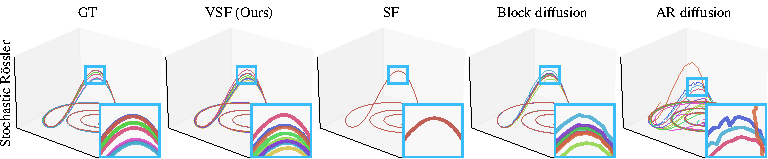
\includegraphics[trim={0bp 0bp 0bp 2bp}, clip, width=0.88\linewidth]{figures/zoom_stochastic_rossler.pdf}
\caption{VSF preserves the R\"ossler geometry while capturing variability
across plausible futures. We show $10$ trajectories from each method. Block
diffusion produces less diverse forecasts, while AR diffusion is more prone to
rollout drift.}
  \label{fig:qualitative-stochastic-rossler}
  \label{fig:qualitative-stochastic}
  \vspace{-0.5cm}
\end{figure}

\subsection{Deterministic Forecasting} \label{sec:exp-deterministic}

We evaluate fully observed deterministic forecasting on the double pendulum,
R\"ossler, and Lorenz systems using 1,000-step rollouts. We report CRPS for the
forecast ensemble and RMSE and MAE for its mean; detailed definitions are
provided in App.~\ref{sec:metrics}.

\textbf{VSF produces accurate forecasts with samples concentrated around the
ground-truth trajectory.}
As shown in Table~\ref{tab:forecasting_results}, VSF achieves the lowest CRPS,
RMSE, and MAE across all three systems, while providing up to a $7\times$
speedup over AR diffusion.
The qualitative forecasts in the Appendix
(\cref{fig:main-chaotic-double-pendulum}) further show that its sampled
trajectories remain close to the reference trajectory throughout the rollout.
%
Chronos-2 is less accurate in these experiments. One possible
factor is the short forecasting context of only 10 time steps.
This is consistent with~\citet{zhang2025zero}, who use 512 context points in
their experiments on chaotic systems and report improved zero-shot
forecasting performance for Chronos as the context length increases.


\begin{wrapfigure}[12]{r}{0.51\linewidth}
  % \vspace{-0.8em}
  \vspace{-1.5em}
  \centering
  \begingroup
  \setlength{\tabcolsep}{1pt}
  \renewcommand{\arraystretch}{1.0}
  \newcommand{\stochasticpreview}[1]{%
    \includegraphics[width=0.3\linewidth]{#1}%
  }
  \newcommand{\stochasticpreviewheader}[1]{%
    {\normalfont\scriptsize\shortstack{#1}}%
  }
  \begin{tabular}{@{}*{3}{c}@{}}
    \stochasticpreviewheader{GT}
    & \stochasticpreviewheader{VSF}
    & \stochasticpreviewheader{AR diff.} \\[0.1em]
    \stochasticpreview{figures/lorenz_stochastic/instance_01_stochastic_lorenz_draw_01_gt.pdf}
    & \stochasticpreview{figures/lorenz_stochastic/instance_01_stochastic_lorenz_draw_01_vsf.pdf}
    & \stochasticpreview{figures/lorenz_stochastic/instance_01_stochastic_lorenz_draw_01_ar_diffusion.pdf} \\[0.1em]
    \stochasticpreview{figures/lorenz_stochastic/instance_01_stochastic_lorenz_draw_08_gt.pdf}
    & \stochasticpreview{figures/lorenz_stochastic/instance_01_stochastic_lorenz_draw_08_vsf.pdf}
    & \stochasticpreview{figures/lorenz_stochastic/instance_01_stochastic_lorenz_draw_08_ar_diffusion.pdf}
  \end{tabular}
  \endgroup
    \vspace{-0.2cm}
    \caption{VSF samples remain consistent with the stochastic Lorenz dynamics,
while AR diffusion drifts from the attractor. Two futures are shown.}
  \label{fig:main-stochastic-lorenz-samples}
  \vspace{-0.8em}
\end{wrapfigure}
\textbf{VSF reduces long-horizon drift relative to SF.}
This difference is most apparent on the double pendulum in
\cref{fig:main-rollout-error-curves}. Adding noise to the initial state
of SF reduces the error somewhat, but its forecasts still drift progressively
from the reference trajectory. VSF maintains lower error over the
same rollout. In our implementation, the previous-frame representation is
combined with the latent variable $\vz$ through a weighted sum at the network
bottleneck (see \cref{sec:experimental-setup}). The ablation in
\cref{sec:full-ablation-results} shows that this latent conditioning is important
for the improved long-horizon accuracy.
\vspace{-3mm}





\subsection{Stochastic Forecasting} \label{sec:exp-stochatic}

We evaluate partially observed stochastic forecasting on the R\"ossler and
Lorenz systems. For each initial state, we generate multiple trajectories by
independently sampling an unobserved dynamical parameter. Each trajectory is
deterministic once this parameter is fixed, but the model does not observe it.
The same observed history can therefore lead to different future trajectories,
including trajectories that separate into different dynamical regimes.
%
We evaluate these forecast distributions using conditional mean error (CME),
conditional standard-deviation error (CSE), Wasserstein distance ($W_1$), and
energy distance (ED). For the values reported in our tables, $W_1$ and ED treat
each complete rollout as a single vector, so they compare distributions over
whole trajectories and account for temporal structure. In the rollout-error
plots, $W_1$ and ED are instead computed pointwise in time. Detailed metric
definitions are provided in App.~\ref{sec:metrics}.


\textbf{VSF best matches the conditional distribution of future trajectories.}
As shown in Table~\ref{tab:forecasting_results}, VSF achieves the lowest value
for every metric on both stochastic systems. The trajectory ensembles in
Figures~\ref{fig:qualitative-stochastic} and
\ref{fig:qualitative-stochastic-lorenz} show that VSF captures both the spread
of the reference futures and the geometry of the underlying dynamics. Block
diffusion and DeepAR cover a narrower part of the distribution, while AR
diffusion produces diverse futures but is more prone to rollout drift.
Perturbing the initial state of SF introduces some diversity, but this
inference-time perturbation is not learned by its training objective.
Unperturbed SF produces only a single trajectory, yielding a CSE of $1$.


% \clearpage
%
\begin{wrapfigure}[12]{r}{0.55\linewidth}
  \vspace{-0.8em}
  \centering
  \setlength{\abovecaptionskip}{3pt}
  \captionof{table}{VSF achieves the lowest CME, CSE, and ED on stochastic
  Lorenz over a 2,500-step rollout. AR diffusion produces diverse samples but
  can drift from the system dynamics, as shown in
  \cref{fig:main-stochastic-lorenz-samples}.}
  \label{tab:stochastic-lorenz-2500}

  \begingroup
  \setlength{\tabcolsep}{2pt}
  \resizebox{\linewidth}{!}{%
  \scriptsize
  \begin{tabular}{@{}l*{4}{>{\columncolor{resultLorenzBg}}c}@{}}
  \toprule
  \multicolumn{5}{c}{\cellcolor{gray!10}{Stochastic dynamics}}\\
  & \multicolumn{4}{c}{\cellcolor{resultLorenzBg}{Lorenz}} \\
  \cmidrule(lr){2-5}
  Model & CME $\downarrow$ & CSE $\downarrow$ & $W_1$ $\downarrow$
  & ED $\downarrow$ \\
  \midrule
  Block diffusion
  & \resultpm{0.79}{0.09} & \resultpm{0.66}{0.11}
  & \fullbestresultpm{76.48}{3.20} & \resultpm{34.79}{11.90} \\
  AR diffusion
  & \resultpm{0.62}{0.03} & \resultpm{0.53}{0.03}
  & \resultpm{96.60}{2.48} & \resultpm{12.43}{0.52} \\
  Rectified flow
  & \resultpm{0.77}{0.16} & \resultpm{0.59}{0.21}
  & \resultpm{90.41}{1.75} & \resultpm{39.60}{16.90} \\
  SF (perturb.)
  & \resultpm{1.13}{0.33} & \resultpm{0.70}{0.21}
  & \resultpm{111.95}{22.66} & \resultpm{39.81}{14.86} \\
  VSF
  & \fullbestresultpm{0.56}{0.07} & \fullbestresultpm{0.39}{0.12}
  & \resultpm{85.67}{7.29} & \fullbestresultpm{12.00}{2.67} \\
  \bottomrule
  \end{tabular}%
  }
  \endgroup
  \vspace{-0.8em}
\end{wrapfigure}
%
\textbf{VSF preserves trajectory structure over very long horizons.}
% Table~\ref{tab:stochastic-lorenz-2500} shows 2,500-step Lorenz rollout, VSF achieves the lowest CME, CSE, and
% ED.
For the 2,500-step Lorenz rollout in Table~\ref{tab:stochastic-lorenz-2500}, VSF achieves the lowest CME, CSE, and ED.
AR diffusion also achieves a low ED, but its sampled trajectories drift
from the system dynamics, as shown in
\cref{fig:main-stochastic-lorenz-samples}. Block diffusion reaches a lower
$W_1$, but its higher CSE and ED are consistent with the narrower mode coverage
seen in \cref{fig:qualitative-stochastic-lorenz}. 
In contrast, VSF
samples traverse both lobes of the attractor while preserving its
characteristic geometry.
\par
%\WFclear

\subsection{World Model Predictor}
\label{sec:exp-world-model}

We next evaluate VSF as an action-conditioned predictor in a JEPA-based world
model. The goal is to test whether its physical-time forecasting formulation
can improve prediction and planning in a learned representation space. We
freeze LeWM's pretrained JEPA representation~\citep{assran2023self, maes2026leworldmodel} and
train only the predictor on offline observation--action trajectories, following
the action-conditioned training setup of V-JEPA~2~\citep{assran2025v}. Future
latent states are used as teacher-forced training targets.
%
We compare LeWM's AR predictor with SF and VSF predictors while keeping the
JEPA encoder, CEM planner, and planning budget fixed. We report
latent-trajectory RMSE along the action sequences selected by CEM and planning
success on PushT, Cube, TwoRoom, and Reacher. The learned JEPA representation
also evolves smoothly over time, as illustrated in
\cref{fig:wm-cube-task-035-vsf-latent-trajectory}, making physical-time
prediction a natural fit for this latent space. Details of the
action-conditioned VSF extension are provided in
App.~\ref{sec:wm-vsf-algorithms}.

\textbf{VSF improves both latent prediction and planning success.}
As shown in \cref{tab:world-model-predictor-results}, VSF reduces
latent-trajectory RMSE relative to the AR predictor on all four tasks and
achieves the lowest RMSE on PushT, TwoRoom, and Reacher. It also achieves the
highest planning success on every task, improving average success by $7.34\%$
over the AR predictor. The successful Cube rollout in
\cref{fig:wm-cube-task-035-vsf-latent-trajectory} provides a qualitative
example, with the predicted latent trajectory closely following the ground
truth. VSF retains LeWM's budget of one velocity-field evaluation
per imagined transition.


\begin{table}[t]
\centering
\caption{As a world-model predictor, VSF achieves the highest planning success on all four tasks and the lowest predictor RMSE on three of four tasks. RMSE is measured between predicted and ground-truth latent trajectories along the CEM-selected action sequence.}
\label{tab:world-model-predictor-results}
\begingroup
% \small
\setlength{\tabcolsep}{4pt}
\resizebox{\linewidth}{!}{%
\begin{tabular}{@{}l*{8}{c}@{}}
% \begin{tabular}{@{}l*{2}{>{\columncolor{resultDPBg}}c}*{2}{>{\columncolor{resultRosslerBg}}c}*{2}{>{\columncolor{resultLorenzBg}}c}*{2}{>{\columncolor{resultRuntimeBg}}c}@{}}
\toprule
& \multicolumn{2}{c}{PushT}
& \multicolumn{2}{c}{Cube}
& \multicolumn{2}{c}{TwoRoom}
& \multicolumn{2}{c}{Reacher} \\
\cmidrule(lr){2-3}\cmidrule(lr){4-5}\cmidrule(lr){6-7}\cmidrule(lr){8-9}
Method
& Success & RMSE $\downarrow$
& Success & RMSE $\downarrow$
& Success & RMSE $\downarrow$
& Success & RMSE $\downarrow$ \\
\midrule
AR predictor
& \resultpm{84.7}{4.1} & \resultpm{0.28}{0.01}
& \resultpm{69.3}{2.5} & \resultpm{0.80}{0.05}
& \resultpm{78.7}{9.0} & \resultpm{0.67}{0.03}
& \resultpm{61.3}{8.2} & \resultpm{1.06}{0.01} \\

SF predictor
& \resultpm{88.0}{2.8} & \resultpm{0.30}{0.04}
& \resultpm{76.7}{0.9} & \fullbestresultpm{0.64}{0.02}
& \resultpm{76.7}{8.2} & \resultpm{0.59}{0.05}
& \resultpm{49.3}{5.0} & \resultpm{1.13}{0.03} \\

% \midrule
VSF predictor
& \fullbestresultpm{92.7}{2.5} & \fullbestresultpm{0.27}{0.03}
& \fullbestresultpm{80.0}{1.6} & \resultpm{0.65}{0.08}
& \fullbestresultpm{82.7}{5.0} & \fullbestresultpm{0.58}{0.01}
& \fullbestresultpm{68.0}{0.0} & \fullbestresultpm{1.03}{0.02} \\
\bottomrule
\end{tabular}%
}
\endgroup
\end{table}


\begin{figure}[t]
  \centering
  % 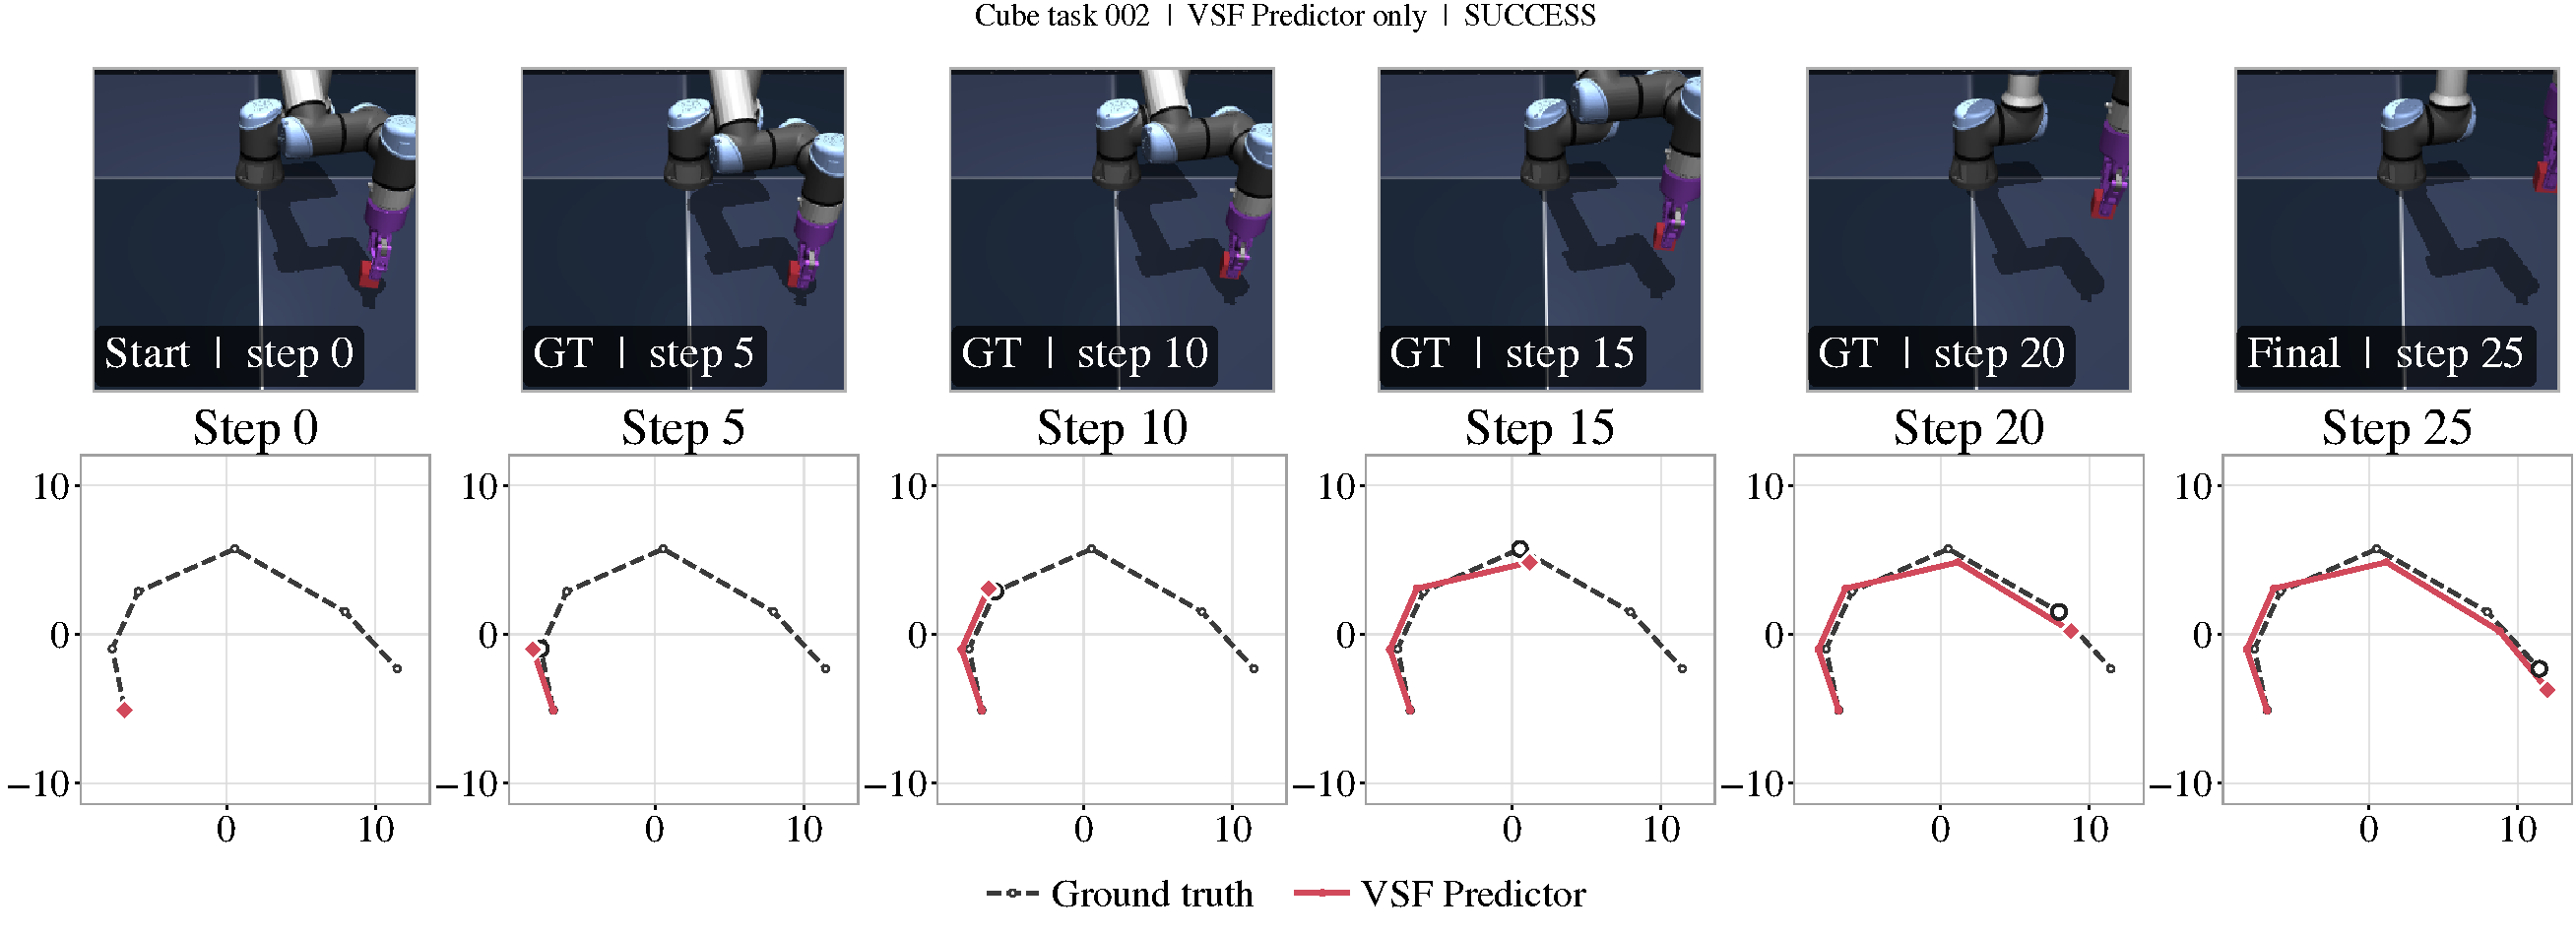
\includegraphics[width=\linewidth, trim={0bp 0bp 0bp 30bp}, clip]{figures/wm/cube_task_002_vsf_latent_trajectory.pdf}
  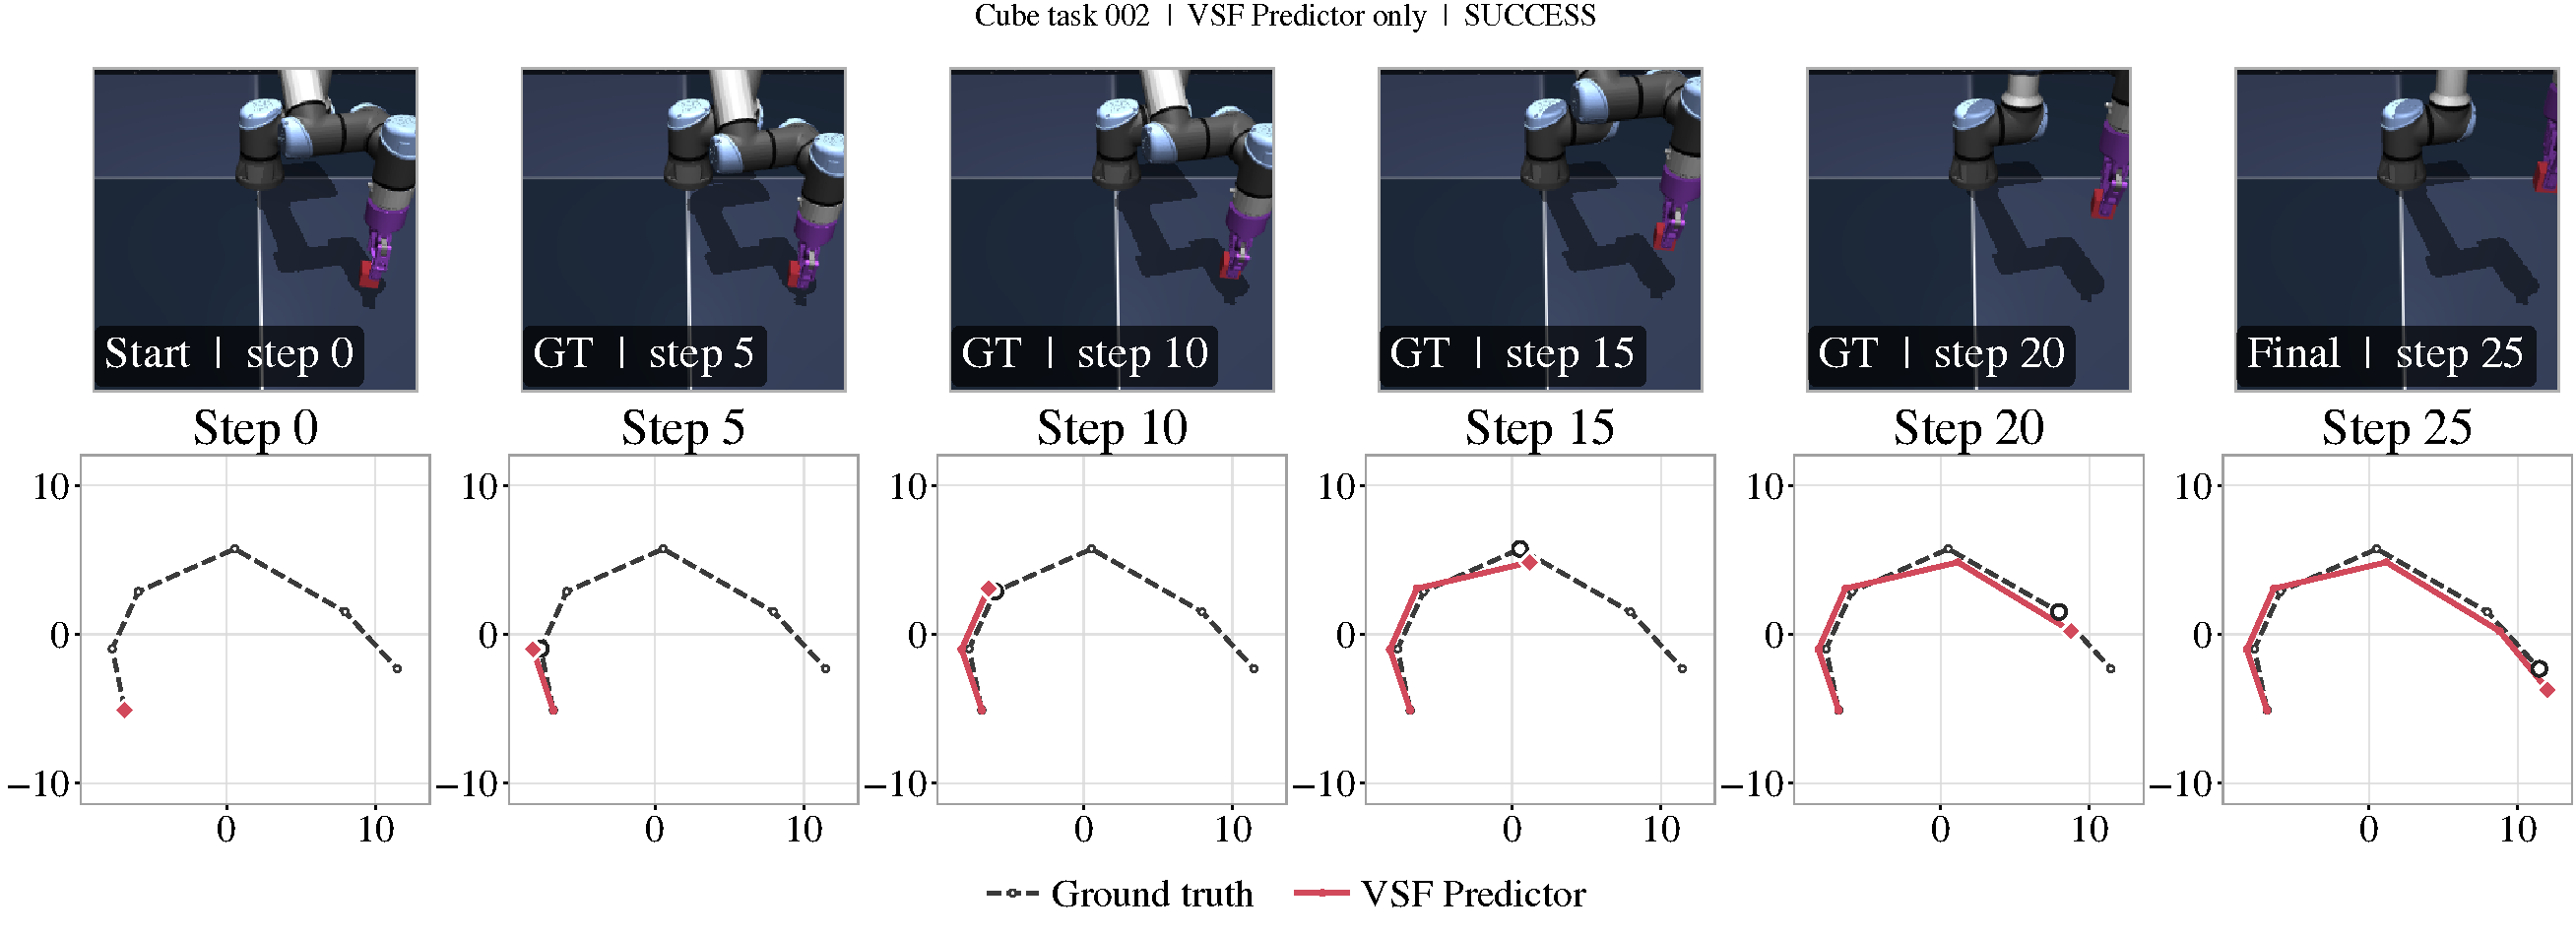
\includegraphics[width=\linewidth, trim={0bp 260bp 0bp 30bp}, clip]{figures/wm/cube_task_002_vsf_latent_trajectory.pdf}
  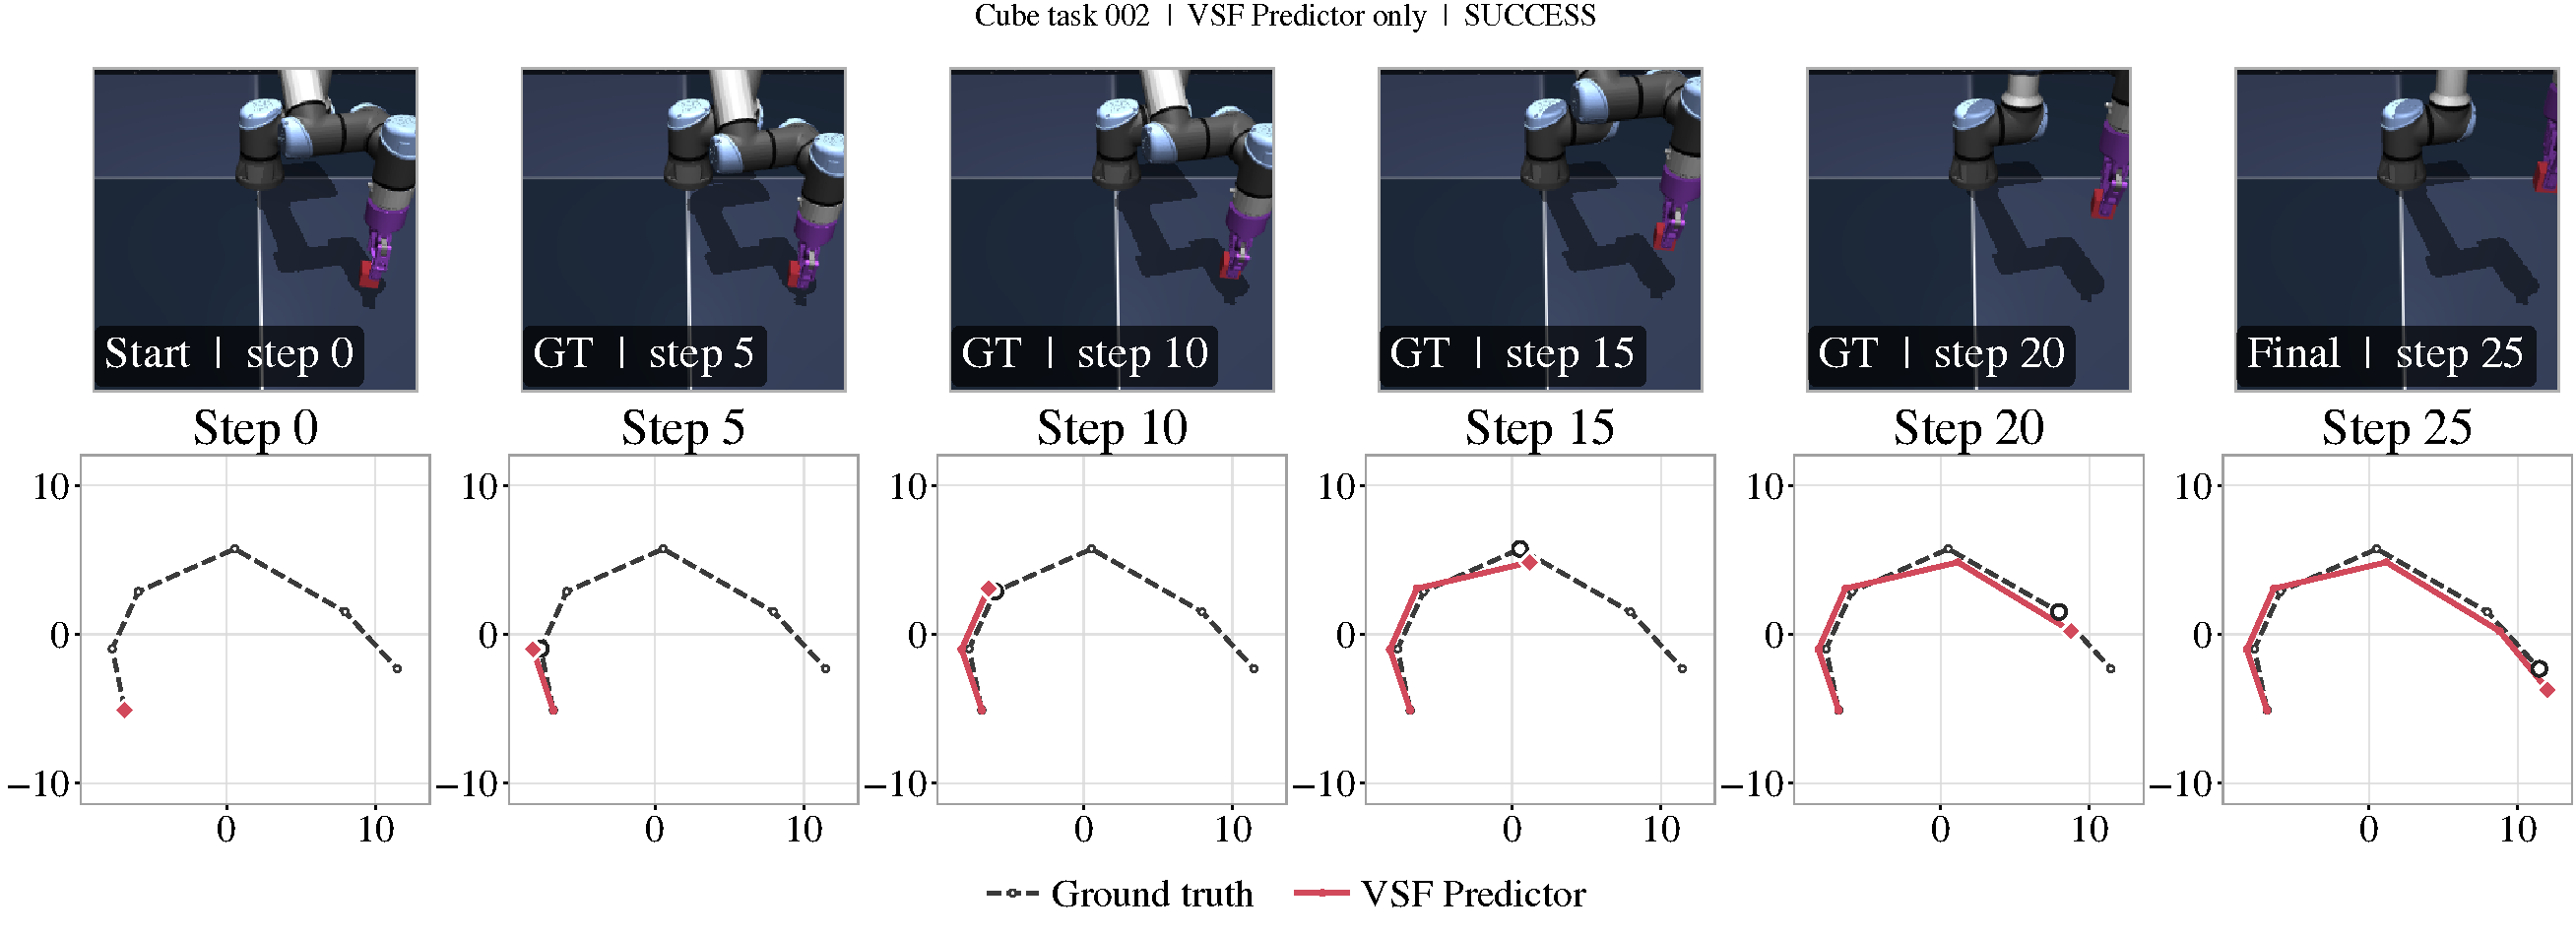
\includegraphics[width=\linewidth, trim={0bp 0bp 0bp 223bp}, clip]{figures/wm/cube_task_002_vsf_latent_trajectory.pdf}
  \vspace{-1.5em}
\caption{VSF serves as an effective world-model predictor on Cube. The top row
shows ground-truth rollout frames, and the bottom row compares the VSF latent
trajectory (red) with the ground truth (dashed). The prediction closely follows
the ground truth and leads to a successful plan.}
  \label{fig:wm-cube-task-035-vsf-latent-trajectory}
    \vspace{-0.2cm}
\end{figure}




\section{Conclusion}

We introduced VSF, a probabilistic extension of SF for forecasting directly in
physical time, where one latent variable conditions an entire rollout. This
allows VSF to model different possible futures while preserving the direct
physical-time generation of SF. We train the latent-conditioned velocity field
with variational inference and an energy-based reconstruction over multiple
latent samples. We also provide a population-level guarantee connecting this
objective to how well the model captures the distribution of possible local
dynamics under prior sampling. Empirically, VSF improves long-horizon
forecasting on deterministic and partially observed stochastic systems,
including the quality of the predicted future distribution, and improves
planning success as an action-conditioned world-model predictor, while
retaining one velocity-field evaluation per imagined transition.

\paragraph{Limitations and future work.} VSF relies on adjacent states providing a meaningful local direction of motion for learning the physical-time velocity. This assumption is most reliable when the dynamics vary smoothly in physical time. Abrupt impacts, discontinuities, or strong observation noise can make the local velocity poorly resolved. VSF also uses explicit forward Euler integration, which can accumulate discretization error for coarse step sizes or rapidly varying learned fields~\citep{hairer1993solving}; solver choice can also affect the effective dynamics learned by neural ODEs~\citep{zhu2022numerical}. Future work could therefore explore hybrid or jump-aware latent dynamics~\citep{jia2019neural},
controlled or rough differential equations~\citep{kidger2020neural,morrill2021neural}, and higher-order or
adaptive Runge--Kutta solvers~\citep{queiruga2020continuous}.


%\section{Conclusion}

%We introduced VSF, a probabilistic physical-time forecasting framework that represents uncertainty through a latent variable conditioning the dynamics and held fixed throughout each rollout.  VSF separates future-specific information from the evolving physical state while retaining the direct physical-time generation of SF. We developed a  variational learning framework with a generalized energy reconstruction for latent-conditioned velocities and established a population energy-distance control result under aggregate posterior--prior alignment. Empirically, VSF improves long-horizon forecasting on deterministic and partially observed stochastic dynamical systems, captures multimodal future trajectories, and improves goal-directed planning when used as an action-conditioned  predictor in world models, while retaining physical-time inference efficiency. 

%More broadly, our results suggest that probabilistic forecasting with generative models can be achieved by modeling uncertainty directly over physical-time dynamics, without introducing a separate generative-time process.


%\section{Limitations and Future Work}
%\label{sec:limitations}

%\paragraph{Temporal regularity.}
%VSF's physical-time alignment is most reliable when adjacent states vary sufficiently smoothly. Under this condition, the previous frame and the adjacent-frame displacement provide an informative local velocity. Abrupt impacts, discontinuities, or severe observation noise can make this direction poorly resolved. Promising extensions include hybrid or jump-aware latent dynamics that separate continuous evolution from discrete events~\citep{jia2019neural}, controlled differential equations that use irregular observations as a driving signal~\citep{kidger2020neural}, and rough differential equations for less regular signals% ~\citep{morrill2021neural}.

%\paragraph{Numerical integration.}
%The reported inference procedures use explicit forward Euler integration. Coarse steps
%or rapidly varying learned fields can accumulate discretization error and may
%produce unstable long rollouts~\citep{hairer1993solving}. The
%choice of solver can affect the effective dynamics learned by a neural
%ODE~\citep{zhu2022numerical}. Future work should compare higher-order and
%adaptive Runge--Kutta methods~\citep{queiruga2020continuous}.









% 
